\documentclass[11pt]{article}
\usepackage[T1]{fontenc}
\usepackage{lmodern}
\usepackage{amsmath,amssymb}
\usepackage{exscale}
\usepackage{tikz}
\usepackage[letterpaper,margin=1.2cm]{geometry}
\pagestyle{empty}
\setlength{\parindent}{0pt}
\begin{document}
{\small Camera-to-LaTeX data sheet. Print at 100\,\%. Photograph each block 3 times with all four corner squares in view; the hollow square goes top left.}\par\vspace{0.3cm}
\begin{center}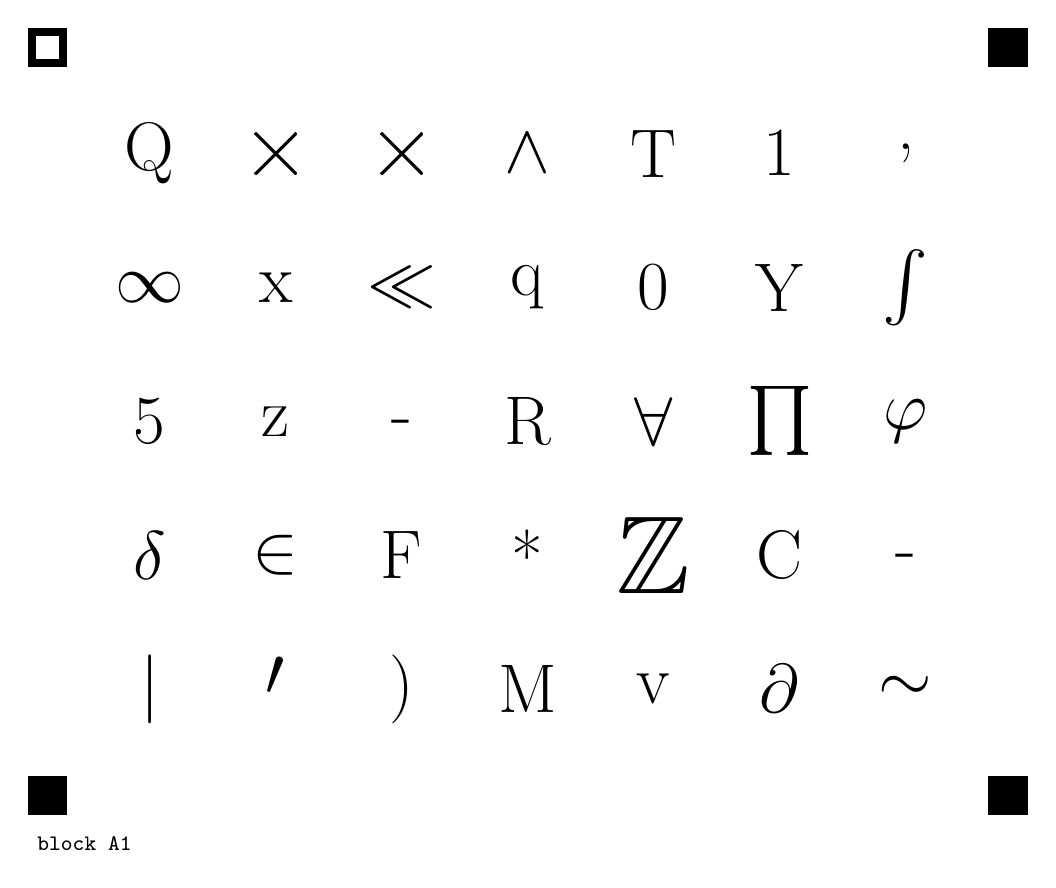
\begin{tikzpicture}[x=1cm,y=-1cm]
\draw[line width=1mm] (-0.700,-0.700) rectangle (-0.300,-0.300);
\fill (11.450,-0.750) rectangle ++(0.500,0.500);
\fill (11.450,8.750) rectangle ++(0.500,0.500);
\fill (-0.750,8.750) rectangle ++(0.500,0.500);
\node[inner sep=0pt] at (0.800,0.850) {\fontsize{40}{48}\selectfont Q};
\node[inner sep=0pt] at (2.400,0.850) {\fontsize{40}{48}\selectfont \texttimes{}};
\node[inner sep=0pt] at (4.000,0.850) {\fontsize{40}{48}\selectfont \texttimes{}};
\node[inner sep=0pt] at (5.600,0.850) {\fontsize{40}{48}\selectfont $\wedge$};
\node[inner sep=0pt] at (7.200,0.850) {\fontsize{40}{48}\selectfont T};
\node[inner sep=0pt] at (8.800,0.850) {\fontsize{40}{48}\selectfont 1};
\node[inner sep=0pt] at (10.400,0.850) {\fontsize{40}{48}\selectfont ,};
\node[inner sep=0pt] at (0.800,2.550) {\fontsize{40}{48}\selectfont $\infty$};
\node[inner sep=0pt] at (2.400,2.550) {\fontsize{40}{48}\selectfont x};
\node[inner sep=0pt] at (4.000,2.550) {\fontsize{40}{48}\selectfont $\ll$};
\node[inner sep=0pt] at (5.600,2.550) {\fontsize{40}{48}\selectfont q};
\node[inner sep=0pt] at (7.200,2.550) {\fontsize{40}{48}\selectfont 0};
\node[inner sep=0pt] at (8.800,2.550) {\fontsize{40}{48}\selectfont Y};
\node[inner sep=0pt] at (10.400,2.550) {\fontsize{40}{48}\selectfont $\int$};
\node[inner sep=0pt] at (0.800,4.250) {\fontsize{40}{48}\selectfont 5};
\node[inner sep=0pt] at (2.400,4.250) {\fontsize{40}{48}\selectfont z};
\node[inner sep=0pt] at (4.000,4.250) {\fontsize{40}{48}\selectfont -};
\node[inner sep=0pt] at (5.600,4.250) {\fontsize{40}{48}\selectfont R};
\node[inner sep=0pt] at (7.200,4.250) {\fontsize{40}{48}\selectfont $\forall$};
\node[inner sep=0pt] at (8.800,4.250) {\fontsize{40}{48}\selectfont $\prod$};
\node[inner sep=0pt] at (10.400,4.250) {\fontsize{40}{48}\selectfont $\varphi$};
\node[inner sep=0pt] at (0.800,5.950) {\fontsize{40}{48}\selectfont $\delta$};
\node[inner sep=0pt] at (2.400,5.950) {\fontsize{40}{48}\selectfont $\in$};
\node[inner sep=0pt] at (4.000,5.950) {\fontsize{40}{48}\selectfont F};
\node[inner sep=0pt] at (5.600,5.950) {\fontsize{40}{48}\selectfont *};
\node[inner sep=0pt] at (7.200,5.950) {\fontsize{40}{48}\selectfont $\mathbb{Z}$};
\node[inner sep=0pt] at (8.800,5.950) {\fontsize{40}{48}\selectfont C};
\node[inner sep=0pt] at (10.400,5.950) {\fontsize{40}{48}\selectfont -};
\node[inner sep=0pt] at (0.800,7.650) {\fontsize{40}{48}\selectfont \textbar{}};
\node[inner sep=0pt] at (2.400,7.650) {\fontsize{40}{48}\selectfont $'$};
\node[inner sep=0pt] at (4.000,7.650) {\fontsize{40}{48}\selectfont )};
\node[inner sep=0pt] at (5.600,7.650) {\fontsize{40}{48}\selectfont M};
\node[inner sep=0pt] at (7.200,7.650) {\fontsize{40}{48}\selectfont v};
\node[inner sep=0pt] at (8.800,7.650) {\fontsize{40}{48}\selectfont $\partial$};
\node[inner sep=0pt] at (10.400,7.650) {\fontsize{40}{48}\selectfont $\sim$};
\node[anchor=north west,font=\footnotesize\ttfamily] at (-0.750,9.400) {block A1};
\end{tikzpicture}\end{center}\vspace{0.2cm}
\begin{center}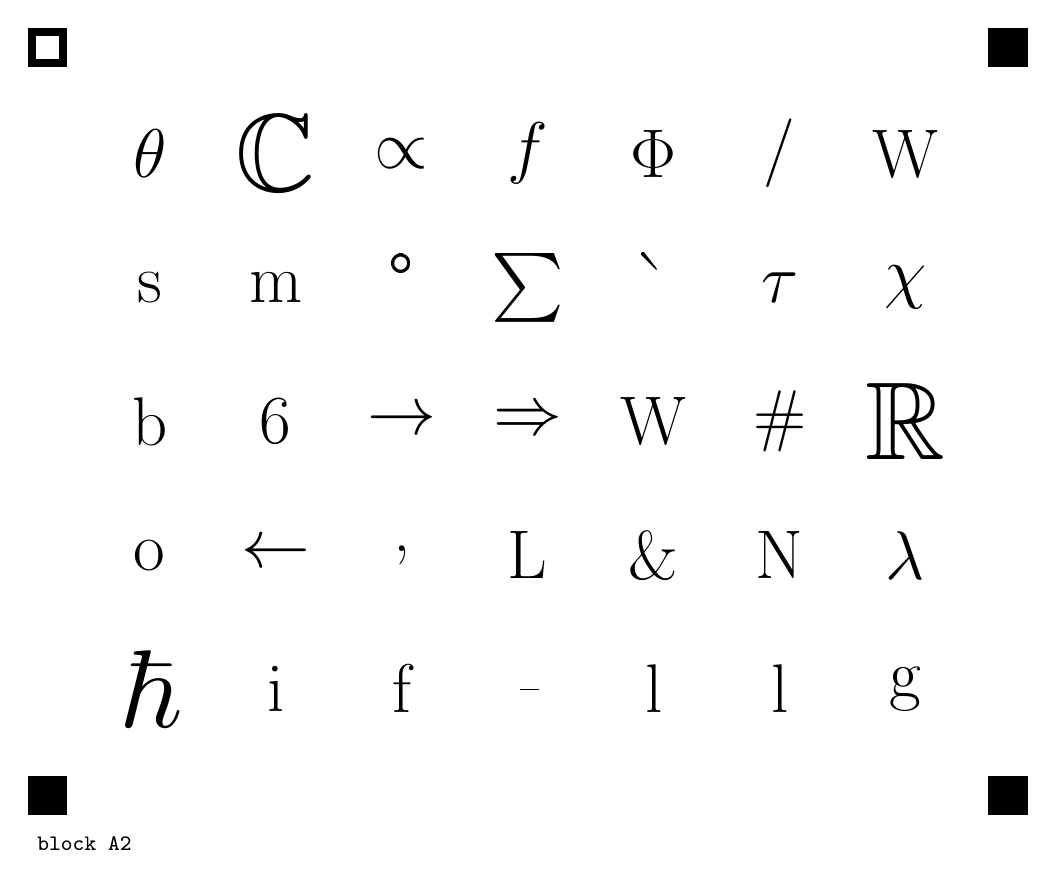
\begin{tikzpicture}[x=1cm,y=-1cm]
\draw[line width=1mm] (-0.700,-0.700) rectangle (-0.300,-0.300);
\fill (11.450,-0.750) rectangle ++(0.500,0.500);
\fill (11.450,8.750) rectangle ++(0.500,0.500);
\fill (-0.750,8.750) rectangle ++(0.500,0.500);
\node[inner sep=0pt] at (0.800,0.850) {\fontsize{40}{48}\selectfont $\theta$};
\node[inner sep=0pt] at (2.400,0.850) {\fontsize{40}{48}\selectfont $\mathbb{C}$};
\node[inner sep=0pt] at (4.000,0.850) {\fontsize{40}{48}\selectfont $\propto$};
\node[inner sep=0pt] at (5.600,0.850) {\fontsize{40}{48}\selectfont $f$};
\node[inner sep=0pt] at (7.200,0.850) {\fontsize{40}{48}\selectfont $\Phi$};
\node[inner sep=0pt] at (8.800,0.850) {\fontsize{40}{48}\selectfont /};
\node[inner sep=0pt] at (10.400,0.850) {\fontsize{40}{48}\selectfont W};
\node[inner sep=0pt] at (0.800,2.550) {\fontsize{40}{48}\selectfont s};
\node[inner sep=0pt] at (2.400,2.550) {\fontsize{40}{48}\selectfont m};
\node[inner sep=0pt] at (4.000,2.550) {\fontsize{40}{48}\selectfont \textdegree{}};
\node[inner sep=0pt] at (5.600,2.550) {\fontsize{40}{48}\selectfont $\sum$};
\node[inner sep=0pt] at (7.200,2.550) {\fontsize{40}{48}\selectfont \textasciigrave{}};
\node[inner sep=0pt] at (8.800,2.550) {\fontsize{40}{48}\selectfont $\tau$};
\node[inner sep=0pt] at (10.400,2.550) {\fontsize{40}{48}\selectfont $\chi$};
\node[inner sep=0pt] at (0.800,4.250) {\fontsize{40}{48}\selectfont b};
\node[inner sep=0pt] at (2.400,4.250) {\fontsize{40}{48}\selectfont 6};
\node[inner sep=0pt] at (4.000,4.250) {\fontsize{40}{48}\selectfont $\rightarrow$};
\node[inner sep=0pt] at (5.600,4.250) {\fontsize{40}{48}\selectfont $\Rightarrow$};
\node[inner sep=0pt] at (7.200,4.250) {\fontsize{40}{48}\selectfont W};
\node[inner sep=0pt] at (8.800,4.250) {\fontsize{40}{48}\selectfont \#};
\node[inner sep=0pt] at (10.400,4.250) {\fontsize{40}{48}\selectfont $\mathbb{R}$};
\node[inner sep=0pt] at (0.800,5.950) {\fontsize{40}{48}\selectfont o};
\node[inner sep=0pt] at (2.400,5.950) {\fontsize{40}{48}\selectfont $\leftarrow$};
\node[inner sep=0pt] at (4.000,5.950) {\fontsize{40}{48}\selectfont ,};
\node[inner sep=0pt] at (5.600,5.950) {\fontsize{40}{48}\selectfont L};
\node[inner sep=0pt] at (7.200,5.950) {\fontsize{40}{48}\selectfont \&};
\node[inner sep=0pt] at (8.800,5.950) {\fontsize{40}{48}\selectfont N};
\node[inner sep=0pt] at (10.400,5.950) {\fontsize{40}{48}\selectfont $\lambda$};
\node[inner sep=0pt] at (0.800,7.650) {\fontsize{40}{48}\selectfont $\hbar$};
\node[inner sep=0pt] at (2.400,7.650) {\fontsize{40}{48}\selectfont i};
\node[inner sep=0pt] at (4.000,7.650) {\fontsize{40}{48}\selectfont f};
\node[inner sep=0pt] at (5.600,7.650) {\fontsize{40}{48}\selectfont \_};
\node[inner sep=0pt] at (7.200,7.650) {\fontsize{40}{48}\selectfont l};
\node[inner sep=0pt] at (8.800,7.650) {\fontsize{40}{48}\selectfont l};
\node[inner sep=0pt] at (10.400,7.650) {\fontsize{40}{48}\selectfont g};
\node[anchor=north west,font=\footnotesize\ttfamily] at (-0.750,9.400) {block A2};
\end{tikzpicture}\end{center}\vspace{0.2cm}
\newpage
{\small Camera-to-LaTeX data sheet. Print at 100\,\%. Photograph each block 3 times with all four corner squares in view; the hollow square goes top left.}\par\vspace{0.3cm}
\begin{center}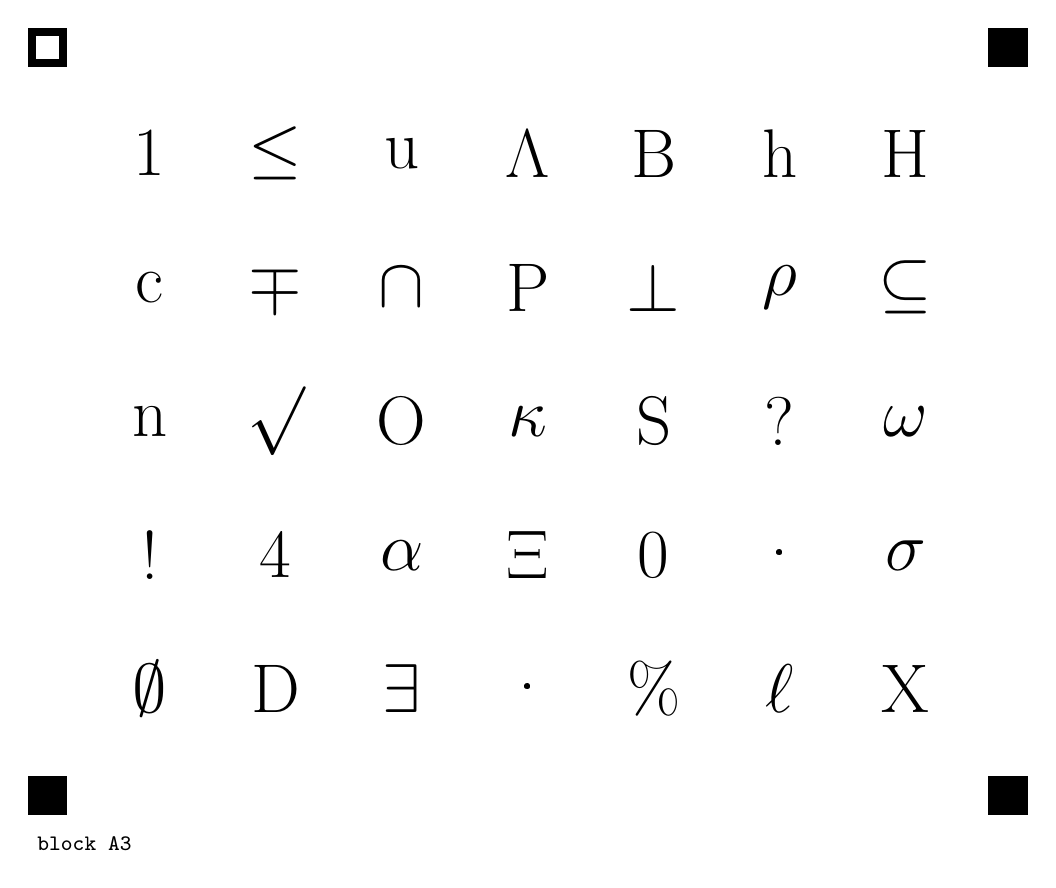
\begin{tikzpicture}[x=1cm,y=-1cm]
\draw[line width=1mm] (-0.700,-0.700) rectangle (-0.300,-0.300);
\fill (11.450,-0.750) rectangle ++(0.500,0.500);
\fill (11.450,8.750) rectangle ++(0.500,0.500);
\fill (-0.750,8.750) rectangle ++(0.500,0.500);
\node[inner sep=0pt] at (0.800,0.850) {\fontsize{40}{48}\selectfont 1};
\node[inner sep=0pt] at (2.400,0.850) {\fontsize{40}{48}\selectfont $\leq$};
\node[inner sep=0pt] at (4.000,0.850) {\fontsize{40}{48}\selectfont u};
\node[inner sep=0pt] at (5.600,0.850) {\fontsize{40}{48}\selectfont $\Lambda$};
\node[inner sep=0pt] at (7.200,0.850) {\fontsize{40}{48}\selectfont B};
\node[inner sep=0pt] at (8.800,0.850) {\fontsize{40}{48}\selectfont h};
\node[inner sep=0pt] at (10.400,0.850) {\fontsize{40}{48}\selectfont H};
\node[inner sep=0pt] at (0.800,2.550) {\fontsize{40}{48}\selectfont c};
\node[inner sep=0pt] at (2.400,2.550) {\fontsize{40}{48}\selectfont $\mp$};
\node[inner sep=0pt] at (4.000,2.550) {\fontsize{40}{48}\selectfont $\cap$};
\node[inner sep=0pt] at (5.600,2.550) {\fontsize{40}{48}\selectfont P};
\node[inner sep=0pt] at (7.200,2.550) {\fontsize{40}{48}\selectfont $\perp$};
\node[inner sep=0pt] at (8.800,2.550) {\fontsize{40}{48}\selectfont $\rho$};
\node[inner sep=0pt] at (10.400,2.550) {\fontsize{40}{48}\selectfont $\subseteq$};
\node[inner sep=0pt] at (0.800,4.250) {\fontsize{40}{48}\selectfont n};
\node[inner sep=0pt] at (2.400,4.250) {\fontsize{40}{48}\selectfont $\surd$};
\node[inner sep=0pt] at (4.000,4.250) {\fontsize{40}{48}\selectfont O};
\node[inner sep=0pt] at (5.600,4.250) {\fontsize{40}{48}\selectfont $\kappa$};
\node[inner sep=0pt] at (7.200,4.250) {\fontsize{40}{48}\selectfont S};
\node[inner sep=0pt] at (8.800,4.250) {\fontsize{40}{48}\selectfont ?};
\node[inner sep=0pt] at (10.400,4.250) {\fontsize{40}{48}\selectfont $\omega$};
\node[inner sep=0pt] at (0.800,5.950) {\fontsize{40}{48}\selectfont !};
\node[inner sep=0pt] at (2.400,5.950) {\fontsize{40}{48}\selectfont 4};
\node[inner sep=0pt] at (4.000,5.950) {\fontsize{40}{48}\selectfont $\alpha$};
\node[inner sep=0pt] at (5.600,5.950) {\fontsize{40}{48}\selectfont $\Xi$};
\node[inner sep=0pt] at (7.200,5.950) {\fontsize{40}{48}\selectfont 0};
\node[inner sep=0pt] at (8.800,5.950) {\fontsize{40}{48}\selectfont \textperiodcentered{}};
\node[inner sep=0pt] at (10.400,5.950) {\fontsize{40}{48}\selectfont $\sigma$};
\node[inner sep=0pt] at (0.800,7.650) {\fontsize{40}{48}\selectfont $\emptyset$};
\node[inner sep=0pt] at (2.400,7.650) {\fontsize{40}{48}\selectfont D};
\node[inner sep=0pt] at (4.000,7.650) {\fontsize{40}{48}\selectfont $\exists$};
\node[inner sep=0pt] at (5.600,7.650) {\fontsize{40}{48}\selectfont \textperiodcentered{}};
\node[inner sep=0pt] at (7.200,7.650) {\fontsize{40}{48}\selectfont \%};
\node[inner sep=0pt] at (8.800,7.650) {\fontsize{40}{48}\selectfont $\ell$};
\node[inner sep=0pt] at (10.400,7.650) {\fontsize{40}{48}\selectfont X};
\node[anchor=north west,font=\footnotesize\ttfamily] at (-0.750,9.400) {block A3};
\end{tikzpicture}\end{center}\vspace{0.2cm}
\begin{center}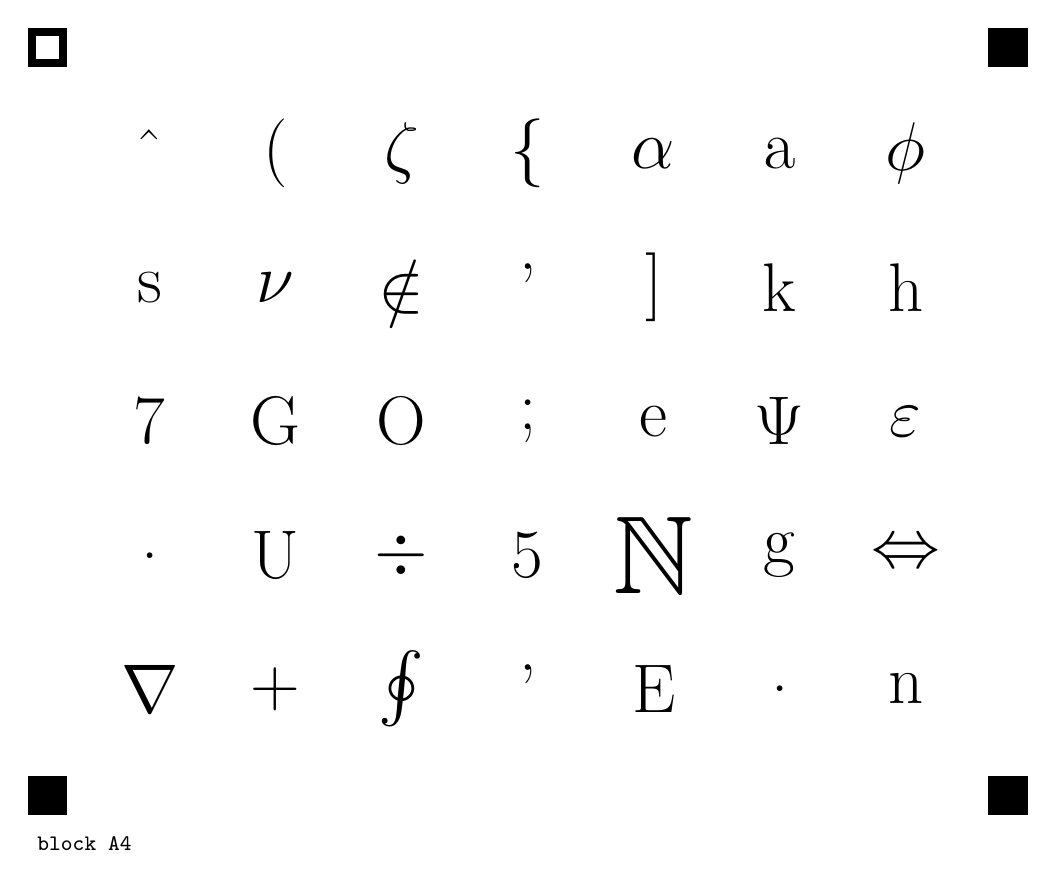
\begin{tikzpicture}[x=1cm,y=-1cm]
\draw[line width=1mm] (-0.700,-0.700) rectangle (-0.300,-0.300);
\fill (11.450,-0.750) rectangle ++(0.500,0.500);
\fill (11.450,8.750) rectangle ++(0.500,0.500);
\fill (-0.750,8.750) rectangle ++(0.500,0.500);
\node[inner sep=0pt] at (0.800,0.850) {\fontsize{40}{48}\selectfont \textasciicircum{}};
\node[inner sep=0pt] at (2.400,0.850) {\fontsize{40}{48}\selectfont (};
\node[inner sep=0pt] at (4.000,0.850) {\fontsize{40}{48}\selectfont $\zeta$};
\node[inner sep=0pt] at (5.600,0.850) {\fontsize{40}{48}\selectfont \{};
\node[inner sep=0pt] at (7.200,0.850) {\fontsize{40}{48}\selectfont $\alpha$};
\node[inner sep=0pt] at (8.800,0.850) {\fontsize{40}{48}\selectfont a};
\node[inner sep=0pt] at (10.400,0.850) {\fontsize{40}{48}\selectfont $\phi$};
\node[inner sep=0pt] at (0.800,2.550) {\fontsize{40}{48}\selectfont s};
\node[inner sep=0pt] at (2.400,2.550) {\fontsize{40}{48}\selectfont $\nu$};
\node[inner sep=0pt] at (4.000,2.550) {\fontsize{40}{48}\selectfont $\notin$};
\node[inner sep=0pt] at (5.600,2.550) {\fontsize{40}{48}\selectfont '};
\node[inner sep=0pt] at (7.200,2.550) {\fontsize{40}{48}\selectfont ]};
\node[inner sep=0pt] at (8.800,2.550) {\fontsize{40}{48}\selectfont k};
\node[inner sep=0pt] at (10.400,2.550) {\fontsize{40}{48}\selectfont h};
\node[inner sep=0pt] at (0.800,4.250) {\fontsize{40}{48}\selectfont 7};
\node[inner sep=0pt] at (2.400,4.250) {\fontsize{40}{48}\selectfont G};
\node[inner sep=0pt] at (4.000,4.250) {\fontsize{40}{48}\selectfont O};
\node[inner sep=0pt] at (5.600,4.250) {\fontsize{40}{48}\selectfont ;};
\node[inner sep=0pt] at (7.200,4.250) {\fontsize{40}{48}\selectfont e};
\node[inner sep=0pt] at (8.800,4.250) {\fontsize{40}{48}\selectfont $\Psi$};
\node[inner sep=0pt] at (10.400,4.250) {\fontsize{40}{48}\selectfont $\varepsilon$};
\node[inner sep=0pt] at (0.800,5.950) {\fontsize{40}{48}\selectfont .};
\node[inner sep=0pt] at (2.400,5.950) {\fontsize{40}{48}\selectfont U};
\node[inner sep=0pt] at (4.000,5.950) {\fontsize{40}{48}\selectfont $\div$};
\node[inner sep=0pt] at (5.600,5.950) {\fontsize{40}{48}\selectfont 5};
\node[inner sep=0pt] at (7.200,5.950) {\fontsize{40}{48}\selectfont $\mathbb{N}$};
\node[inner sep=0pt] at (8.800,5.950) {\fontsize{40}{48}\selectfont g};
\node[inner sep=0pt] at (10.400,5.950) {\fontsize{40}{48}\selectfont $\Leftrightarrow$};
\node[inner sep=0pt] at (0.800,7.650) {\fontsize{40}{48}\selectfont $\nabla$};
\node[inner sep=0pt] at (2.400,7.650) {\fontsize{40}{48}\selectfont +};
\node[inner sep=0pt] at (4.000,7.650) {\fontsize{40}{48}\selectfont $\oint$};
\node[inner sep=0pt] at (5.600,7.650) {\fontsize{40}{48}\selectfont '};
\node[inner sep=0pt] at (7.200,7.650) {\fontsize{40}{48}\selectfont E};
\node[inner sep=0pt] at (8.800,7.650) {\fontsize{40}{48}\selectfont .};
\node[inner sep=0pt] at (10.400,7.650) {\fontsize{40}{48}\selectfont n};
\node[anchor=north west,font=\footnotesize\ttfamily] at (-0.750,9.400) {block A4};
\end{tikzpicture}\end{center}\vspace{0.2cm}
\newpage
{\small Camera-to-LaTeX data sheet. Print at 100\,\%. Photograph each block 3 times with all four corner squares in view; the hollow square goes top left.}\par\vspace{0.3cm}
\begin{center}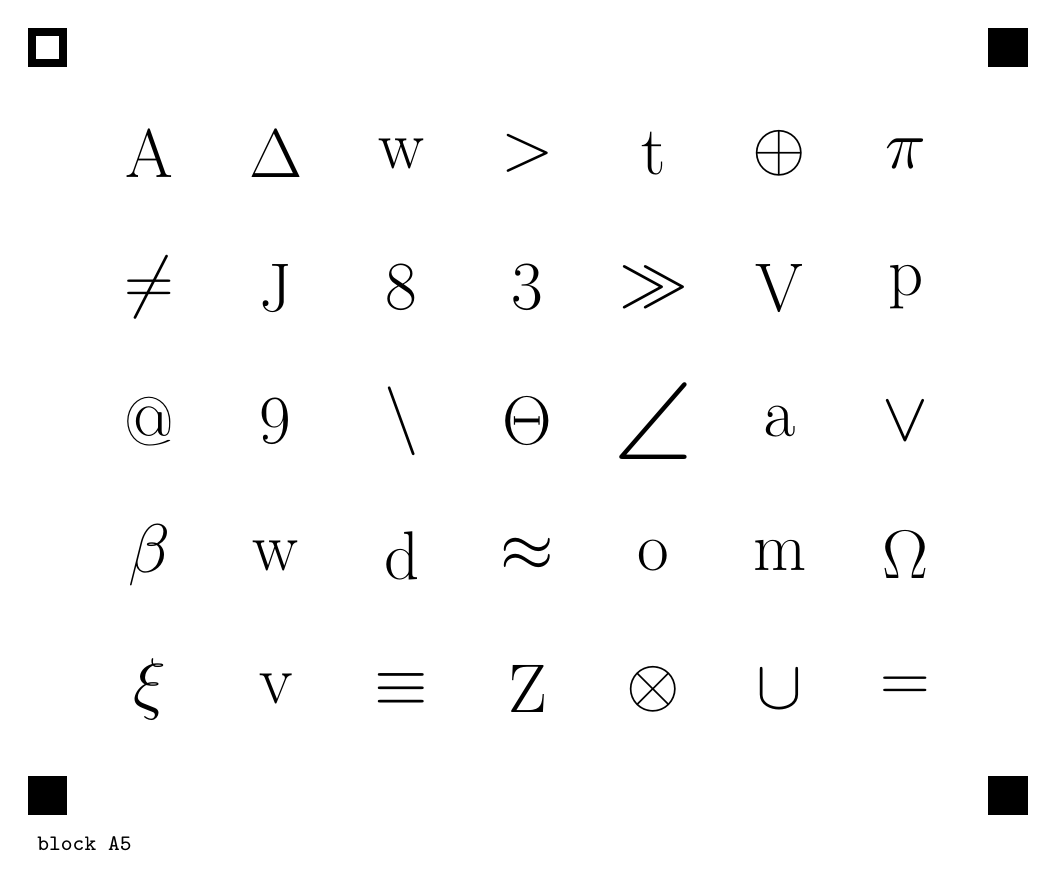
\begin{tikzpicture}[x=1cm,y=-1cm]
\draw[line width=1mm] (-0.700,-0.700) rectangle (-0.300,-0.300);
\fill (11.450,-0.750) rectangle ++(0.500,0.500);
\fill (11.450,8.750) rectangle ++(0.500,0.500);
\fill (-0.750,8.750) rectangle ++(0.500,0.500);
\node[inner sep=0pt] at (0.800,0.850) {\fontsize{40}{48}\selectfont A};
\node[inner sep=0pt] at (2.400,0.850) {\fontsize{40}{48}\selectfont $\Delta$};
\node[inner sep=0pt] at (4.000,0.850) {\fontsize{40}{48}\selectfont w};
\node[inner sep=0pt] at (5.600,0.850) {\fontsize{40}{48}\selectfont \textgreater{}};
\node[inner sep=0pt] at (7.200,0.850) {\fontsize{40}{48}\selectfont t};
\node[inner sep=0pt] at (8.800,0.850) {\fontsize{40}{48}\selectfont $\oplus$};
\node[inner sep=0pt] at (10.400,0.850) {\fontsize{40}{48}\selectfont $\pi$};
\node[inner sep=0pt] at (0.800,2.550) {\fontsize{40}{48}\selectfont $\neq$};
\node[inner sep=0pt] at (2.400,2.550) {\fontsize{40}{48}\selectfont J};
\node[inner sep=0pt] at (4.000,2.550) {\fontsize{40}{48}\selectfont 8};
\node[inner sep=0pt] at (5.600,2.550) {\fontsize{40}{48}\selectfont 3};
\node[inner sep=0pt] at (7.200,2.550) {\fontsize{40}{48}\selectfont $\gg$};
\node[inner sep=0pt] at (8.800,2.550) {\fontsize{40}{48}\selectfont V};
\node[inner sep=0pt] at (10.400,2.550) {\fontsize{40}{48}\selectfont p};
\node[inner sep=0pt] at (0.800,4.250) {\fontsize{40}{48}\selectfont @};
\node[inner sep=0pt] at (2.400,4.250) {\fontsize{40}{48}\selectfont 9};
\node[inner sep=0pt] at (4.000,4.250) {\fontsize{40}{48}\selectfont \textbackslash{}};
\node[inner sep=0pt] at (5.600,4.250) {\fontsize{40}{48}\selectfont $\Theta$};
\node[inner sep=0pt] at (7.200,4.250) {\fontsize{40}{48}\selectfont $\angle$};
\node[inner sep=0pt] at (8.800,4.250) {\fontsize{40}{48}\selectfont a};
\node[inner sep=0pt] at (10.400,4.250) {\fontsize{40}{48}\selectfont $\vee$};
\node[inner sep=0pt] at (0.800,5.950) {\fontsize{40}{48}\selectfont $\beta$};
\node[inner sep=0pt] at (2.400,5.950) {\fontsize{40}{48}\selectfont w};
\node[inner sep=0pt] at (4.000,5.950) {\fontsize{40}{48}\selectfont d};
\node[inner sep=0pt] at (5.600,5.950) {\fontsize{40}{48}\selectfont $\approx$};
\node[inner sep=0pt] at (7.200,5.950) {\fontsize{40}{48}\selectfont o};
\node[inner sep=0pt] at (8.800,5.950) {\fontsize{40}{48}\selectfont m};
\node[inner sep=0pt] at (10.400,5.950) {\fontsize{40}{48}\selectfont $\Omega$};
\node[inner sep=0pt] at (0.800,7.650) {\fontsize{40}{48}\selectfont $\xi$};
\node[inner sep=0pt] at (2.400,7.650) {\fontsize{40}{48}\selectfont v};
\node[inner sep=0pt] at (4.000,7.650) {\fontsize{40}{48}\selectfont $\equiv$};
\node[inner sep=0pt] at (5.600,7.650) {\fontsize{40}{48}\selectfont Z};
\node[inner sep=0pt] at (7.200,7.650) {\fontsize{40}{48}\selectfont $\otimes$};
\node[inner sep=0pt] at (8.800,7.650) {\fontsize{40}{48}\selectfont $\cup$};
\node[inner sep=0pt] at (10.400,7.650) {\fontsize{40}{48}\selectfont =};
\node[anchor=north west,font=\footnotesize\ttfamily] at (-0.750,9.400) {block A5};
\end{tikzpicture}\end{center}\vspace{0.2cm}
\begin{center}\begin{tikzpicture}[x=1cm,y=-1cm]
\draw[line width=1mm] (-0.700,-0.700) rectangle (-0.300,-0.300);
\fill (11.450,-0.750) rectangle ++(0.500,0.500);
\fill (11.450,8.750) rectangle ++(0.500,0.500);
\fill (-0.750,8.750) rectangle ++(0.500,0.500);
\node[inner sep=0pt] at (0.800,0.850) {\fontsize{40}{48}\selectfont $\mu$};
\node[inner sep=0pt] at (2.400,0.850) {\fontsize{40}{48}\selectfont \}};
\node[inner sep=0pt] at (4.000,0.850) {\fontsize{40}{48}\selectfont I};
\node[inner sep=0pt] at (5.600,0.850) {\fontsize{40}{48}\selectfont $\geq$};
\node[inner sep=0pt] at (7.200,0.850) {\fontsize{40}{48}\selectfont $\psi$};
\node[inner sep=0pt] at (8.800,0.850) {\fontsize{40}{48}\selectfont [};
\node[inner sep=0pt] at (10.400,0.850) {\fontsize{40}{48}\selectfont $\parallel$};
\node[inner sep=0pt] at (0.800,2.550) {\fontsize{40}{48}\selectfont r};
\node[inner sep=0pt] at (2.400,2.550) {\fontsize{40}{48}\selectfont y};
\node[inner sep=0pt] at (4.000,2.550) {\fontsize{40}{48}\selectfont \textless{}};
\node[inner sep=0pt] at (5.600,2.550) {\fontsize{40}{48}\selectfont K};
\node[inner sep=0pt] at (7.200,2.550) {\fontsize{40}{48}\selectfont $\subset$};
\node[inner sep=0pt] at (8.800,2.550) {\fontsize{40}{48}\selectfont $\mathbb{Q}$};
\node[inner sep=0pt] at (10.400,2.550) {\fontsize{40}{48}\selectfont $\pm$};
\node[inner sep=0pt] at (0.800,4.250) {\fontsize{40}{48}\selectfont \textquotedbl{}};
\node[inner sep=0pt] at (2.400,4.250) {\fontsize{40}{48}\selectfont $\neg$};
\node[inner sep=0pt] at (4.000,4.250) {\fontsize{40}{48}\selectfont x};
\node[inner sep=0pt] at (5.600,4.250) {\fontsize{40}{48}\selectfont y};
\node[inner sep=0pt] at (7.200,4.250) {\fontsize{40}{48}\selectfont $\ast$};
\node[inner sep=0pt] at (8.800,4.250) {\fontsize{40}{48}\selectfont I};
\node[inner sep=0pt] at (10.400,4.250) {\fontsize{40}{48}\selectfont $\Pi$};
\node[inner sep=0pt] at (0.800,5.950) {\fontsize{40}{48}\selectfont 2};
\node[inner sep=0pt] at (2.400,5.950) {\fontsize{40}{48}\selectfont $\leftrightarrow$};
\node[inner sep=0pt] at (4.000,5.950) {\fontsize{40}{48}\selectfont \textasciitilde{}};
\node[inner sep=0pt] at (5.600,5.950) {\fontsize{40}{48}\selectfont $\epsilon$};
\node[inner sep=0pt] at (7.200,5.950) {\fontsize{40}{48}\selectfont :};
\node[inner sep=0pt] at (8.800,5.950) {\fontsize{40}{48}\selectfont u};
\node[inner sep=0pt] at (10.400,5.950) {\fontsize{40}{48}\selectfont $\gamma$};
\node[inner sep=0pt] at (0.800,7.650) {\fontsize{40}{48}\selectfont $\Gamma$};
\node[inner sep=0pt] at (2.400,7.650) {\fontsize{40}{48}\selectfont $\Sigma$};
\node[inner sep=0pt] at (4.000,7.650) {\fontsize{40}{48}\selectfont \$};
\node[inner sep=0pt] at (5.600,7.650) {\fontsize{40}{48}\selectfont j};
\node[inner sep=0pt] at (7.200,7.650) {\fontsize{40}{48}\selectfont $\eta$};
\node[inner sep=0pt] at (8.800,7.650) {\fontsize{40}{48}\selectfont \_};
\node[inner sep=0pt] at (10.400,7.650) {\fontsize{40}{48}\selectfont \textbar{}};
\node[anchor=north west,font=\footnotesize\ttfamily] at (-0.750,9.400) {block A6};
\end{tikzpicture}\end{center}\vspace{0.2cm}
\newpage
{\small Camera-to-LaTeX data sheet. Print at 100\,\%. Photograph each block 3 times with all four corner squares in view; the hollow square goes top left.}\par\vspace{0.3cm}
\begin{center}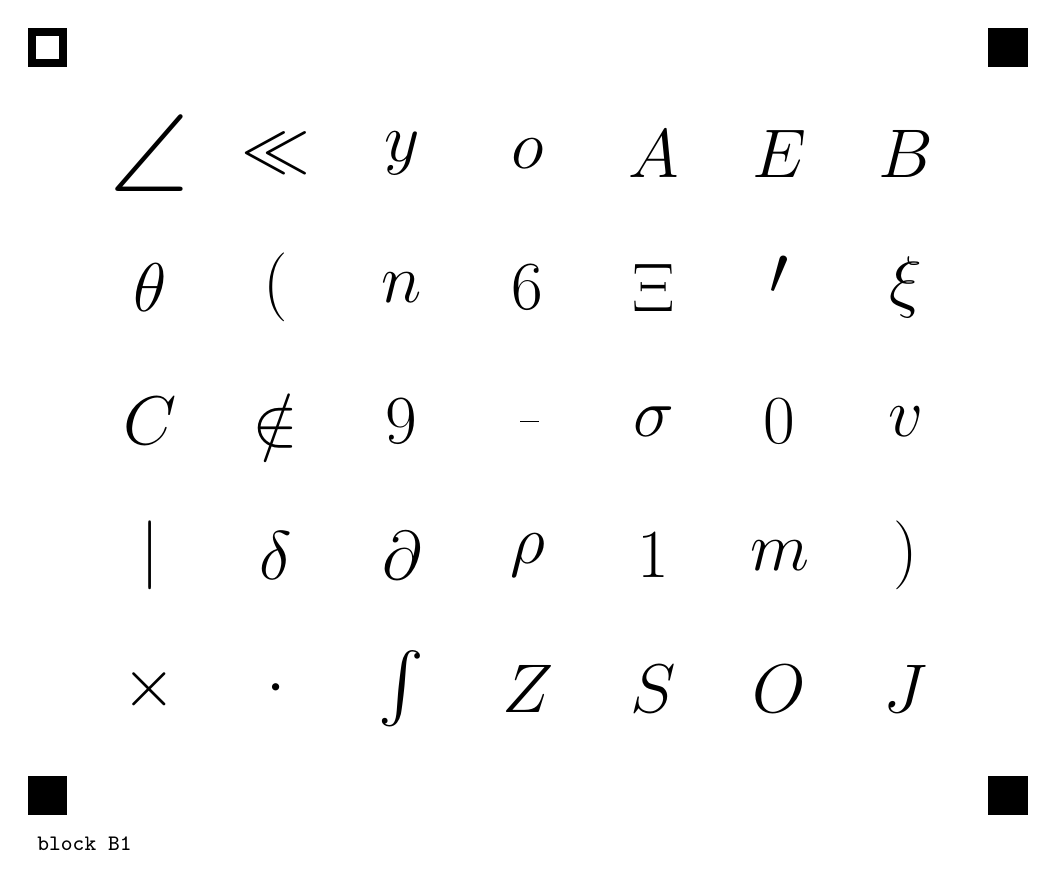
\begin{tikzpicture}[x=1cm,y=-1cm]
\draw[line width=1mm] (-0.700,-0.700) rectangle (-0.300,-0.300);
\fill (11.450,-0.750) rectangle ++(0.500,0.500);
\fill (11.450,8.750) rectangle ++(0.500,0.500);
\fill (-0.750,8.750) rectangle ++(0.500,0.500);
\node[inner sep=0pt] at (0.800,0.850) {\fontsize{40}{48}\selectfont $\angle$};
\node[inner sep=0pt] at (2.400,0.850) {\fontsize{40}{48}\selectfont $\ll$};
\node[inner sep=0pt] at (4.000,0.850) {\fontsize{40}{48}\selectfont $y$};
\node[inner sep=0pt] at (5.600,0.850) {\fontsize{40}{48}\selectfont $o$};
\node[inner sep=0pt] at (7.200,0.850) {\fontsize{40}{48}\selectfont $A$};
\node[inner sep=0pt] at (8.800,0.850) {\fontsize{40}{48}\selectfont $E$};
\node[inner sep=0pt] at (10.400,0.850) {\fontsize{40}{48}\selectfont $B$};
\node[inner sep=0pt] at (0.800,2.550) {\fontsize{40}{48}\selectfont $\theta$};
\node[inner sep=0pt] at (2.400,2.550) {\fontsize{40}{48}\selectfont $($};
\node[inner sep=0pt] at (4.000,2.550) {\fontsize{40}{48}\selectfont $n$};
\node[inner sep=0pt] at (5.600,2.550) {\fontsize{40}{48}\selectfont $6$};
\node[inner sep=0pt] at (7.200,2.550) {\fontsize{40}{48}\selectfont $\Xi$};
\node[inner sep=0pt] at (8.800,2.550) {\fontsize{40}{48}\selectfont $'$};
\node[inner sep=0pt] at (10.400,2.550) {\fontsize{40}{48}\selectfont $\xi$};
\node[inner sep=0pt] at (0.800,4.250) {\fontsize{40}{48}\selectfont $C$};
\node[inner sep=0pt] at (2.400,4.250) {\fontsize{40}{48}\selectfont $\notin$};
\node[inner sep=0pt] at (4.000,4.250) {\fontsize{40}{48}\selectfont $9$};
\node[inner sep=0pt] at (5.600,4.250) {\fontsize{40}{48}\selectfont $\_$};
\node[inner sep=0pt] at (7.200,4.250) {\fontsize{40}{48}\selectfont $\sigma$};
\node[inner sep=0pt] at (8.800,4.250) {\fontsize{40}{48}\selectfont $0$};
\node[inner sep=0pt] at (10.400,4.250) {\fontsize{40}{48}\selectfont $v$};
\node[inner sep=0pt] at (0.800,5.950) {\fontsize{40}{48}\selectfont $|$};
\node[inner sep=0pt] at (2.400,5.950) {\fontsize{40}{48}\selectfont $\delta$};
\node[inner sep=0pt] at (4.000,5.950) {\fontsize{40}{48}\selectfont $\partial$};
\node[inner sep=0pt] at (5.600,5.950) {\fontsize{40}{48}\selectfont $\rho$};
\node[inner sep=0pt] at (7.200,5.950) {\fontsize{40}{48}\selectfont $1$};
\node[inner sep=0pt] at (8.800,5.950) {\fontsize{40}{48}\selectfont $m$};
\node[inner sep=0pt] at (10.400,5.950) {\fontsize{40}{48}\selectfont $)$};
\node[inner sep=0pt] at (0.800,7.650) {\fontsize{40}{48}\selectfont $\times$};
\node[inner sep=0pt] at (2.400,7.650) {\fontsize{40}{48}\selectfont $\cdot$};
\node[inner sep=0pt] at (4.000,7.650) {\fontsize{40}{48}\selectfont $\int$};
\node[inner sep=0pt] at (5.600,7.650) {\fontsize{40}{48}\selectfont $Z$};
\node[inner sep=0pt] at (7.200,7.650) {\fontsize{40}{48}\selectfont $S$};
\node[inner sep=0pt] at (8.800,7.650) {\fontsize{40}{48}\selectfont $O$};
\node[inner sep=0pt] at (10.400,7.650) {\fontsize{40}{48}\selectfont $J$};
\node[anchor=north west,font=\footnotesize\ttfamily] at (-0.750,9.400) {block B1};
\end{tikzpicture}\end{center}\vspace{0.2cm}
\begin{center}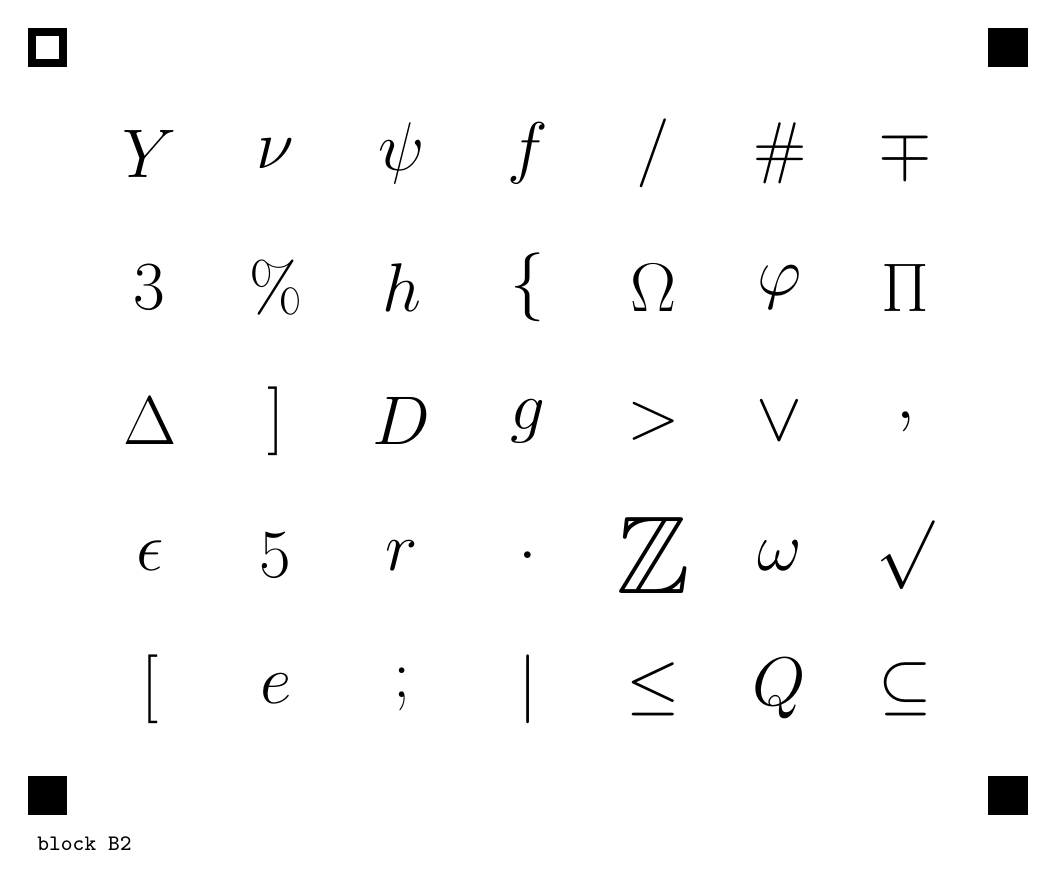
\begin{tikzpicture}[x=1cm,y=-1cm]
\draw[line width=1mm] (-0.700,-0.700) rectangle (-0.300,-0.300);
\fill (11.450,-0.750) rectangle ++(0.500,0.500);
\fill (11.450,8.750) rectangle ++(0.500,0.500);
\fill (-0.750,8.750) rectangle ++(0.500,0.500);
\node[inner sep=0pt] at (0.800,0.850) {\fontsize{40}{48}\selectfont $Y$};
\node[inner sep=0pt] at (2.400,0.850) {\fontsize{40}{48}\selectfont $\nu$};
\node[inner sep=0pt] at (4.000,0.850) {\fontsize{40}{48}\selectfont $\psi$};
\node[inner sep=0pt] at (5.600,0.850) {\fontsize{40}{48}\selectfont $f$};
\node[inner sep=0pt] at (7.200,0.850) {\fontsize{40}{48}\selectfont $/$};
\node[inner sep=0pt] at (8.800,0.850) {\fontsize{40}{48}\selectfont $\#$};
\node[inner sep=0pt] at (10.400,0.850) {\fontsize{40}{48}\selectfont $\mp$};
\node[inner sep=0pt] at (0.800,2.550) {\fontsize{40}{48}\selectfont $3$};
\node[inner sep=0pt] at (2.400,2.550) {\fontsize{40}{48}\selectfont $\%$};
\node[inner sep=0pt] at (4.000,2.550) {\fontsize{40}{48}\selectfont $h$};
\node[inner sep=0pt] at (5.600,2.550) {\fontsize{40}{48}\selectfont $\{$};
\node[inner sep=0pt] at (7.200,2.550) {\fontsize{40}{48}\selectfont $\Omega$};
\node[inner sep=0pt] at (8.800,2.550) {\fontsize{40}{48}\selectfont $\varphi$};
\node[inner sep=0pt] at (10.400,2.550) {\fontsize{40}{48}\selectfont $\Pi$};
\node[inner sep=0pt] at (0.800,4.250) {\fontsize{40}{48}\selectfont $\Delta$};
\node[inner sep=0pt] at (2.400,4.250) {\fontsize{40}{48}\selectfont $]$};
\node[inner sep=0pt] at (4.000,4.250) {\fontsize{40}{48}\selectfont $D$};
\node[inner sep=0pt] at (5.600,4.250) {\fontsize{40}{48}\selectfont $g$};
\node[inner sep=0pt] at (7.200,4.250) {\fontsize{40}{48}\selectfont $>$};
\node[inner sep=0pt] at (8.800,4.250) {\fontsize{40}{48}\selectfont $\vee$};
\node[inner sep=0pt] at (10.400,4.250) {\fontsize{40}{48}\selectfont $,$};
\node[inner sep=0pt] at (0.800,5.950) {\fontsize{40}{48}\selectfont $\epsilon$};
\node[inner sep=0pt] at (2.400,5.950) {\fontsize{40}{48}\selectfont $5$};
\node[inner sep=0pt] at (4.000,5.950) {\fontsize{40}{48}\selectfont $r$};
\node[inner sep=0pt] at (5.600,5.950) {\fontsize{40}{48}\selectfont $.$};
\node[inner sep=0pt] at (7.200,5.950) {\fontsize{40}{48}\selectfont $\mathbb{Z}$};
\node[inner sep=0pt] at (8.800,5.950) {\fontsize{40}{48}\selectfont $\omega$};
\node[inner sep=0pt] at (10.400,5.950) {\fontsize{40}{48}\selectfont $\surd$};
\node[inner sep=0pt] at (0.800,7.650) {\fontsize{40}{48}\selectfont $[$};
\node[inner sep=0pt] at (2.400,7.650) {\fontsize{40}{48}\selectfont $e$};
\node[inner sep=0pt] at (4.000,7.650) {\fontsize{40}{48}\selectfont $;$};
\node[inner sep=0pt] at (5.600,7.650) {\fontsize{40}{48}\selectfont $|$};
\node[inner sep=0pt] at (7.200,7.650) {\fontsize{40}{48}\selectfont $\leq$};
\node[inner sep=0pt] at (8.800,7.650) {\fontsize{40}{48}\selectfont $Q$};
\node[inner sep=0pt] at (10.400,7.650) {\fontsize{40}{48}\selectfont $\subseteq$};
\node[anchor=north west,font=\footnotesize\ttfamily] at (-0.750,9.400) {block B2};
\end{tikzpicture}\end{center}\vspace{0.2cm}
\newpage
{\small Camera-to-LaTeX data sheet. Print at 100\,\%. Photograph each block 3 times with all four corner squares in view; the hollow square goes top left.}\par\vspace{0.3cm}
\begin{center}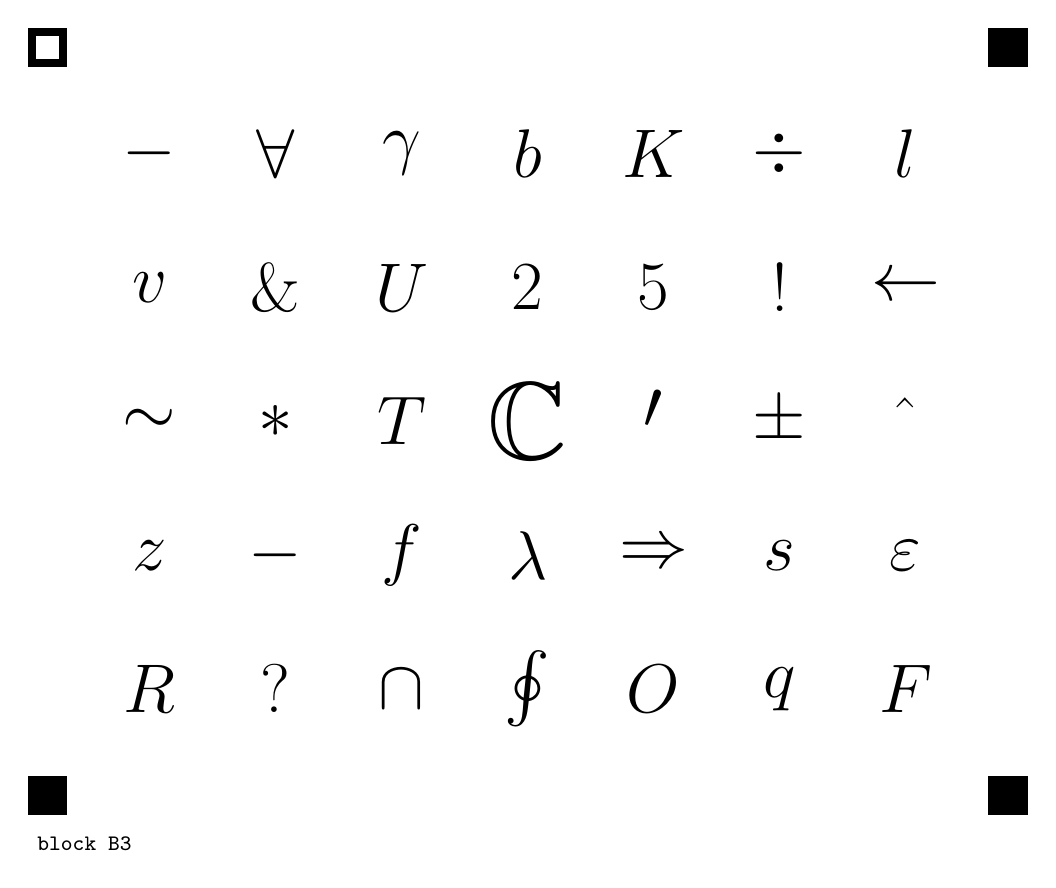
\begin{tikzpicture}[x=1cm,y=-1cm]
\draw[line width=1mm] (-0.700,-0.700) rectangle (-0.300,-0.300);
\fill (11.450,-0.750) rectangle ++(0.500,0.500);
\fill (11.450,8.750) rectangle ++(0.500,0.500);
\fill (-0.750,8.750) rectangle ++(0.500,0.500);
\node[inner sep=0pt] at (0.800,0.850) {\fontsize{40}{48}\selectfont $-$};
\node[inner sep=0pt] at (2.400,0.850) {\fontsize{40}{48}\selectfont $\forall$};
\node[inner sep=0pt] at (4.000,0.850) {\fontsize{40}{48}\selectfont $\gamma$};
\node[inner sep=0pt] at (5.600,0.850) {\fontsize{40}{48}\selectfont $b$};
\node[inner sep=0pt] at (7.200,0.850) {\fontsize{40}{48}\selectfont $K$};
\node[inner sep=0pt] at (8.800,0.850) {\fontsize{40}{48}\selectfont $\div$};
\node[inner sep=0pt] at (10.400,0.850) {\fontsize{40}{48}\selectfont $l$};
\node[inner sep=0pt] at (0.800,2.550) {\fontsize{40}{48}\selectfont $v$};
\node[inner sep=0pt] at (2.400,2.550) {\fontsize{40}{48}\selectfont $\&$};
\node[inner sep=0pt] at (4.000,2.550) {\fontsize{40}{48}\selectfont $U$};
\node[inner sep=0pt] at (5.600,2.550) {\fontsize{40}{48}\selectfont $2$};
\node[inner sep=0pt] at (7.200,2.550) {\fontsize{40}{48}\selectfont $5$};
\node[inner sep=0pt] at (8.800,2.550) {\fontsize{40}{48}\selectfont $!$};
\node[inner sep=0pt] at (10.400,2.550) {\fontsize{40}{48}\selectfont $\leftarrow$};
\node[inner sep=0pt] at (0.800,4.250) {\fontsize{40}{48}\selectfont $\sim$};
\node[inner sep=0pt] at (2.400,4.250) {\fontsize{40}{48}\selectfont $\ast$};
\node[inner sep=0pt] at (4.000,4.250) {\fontsize{40}{48}\selectfont $T$};
\node[inner sep=0pt] at (5.600,4.250) {\fontsize{40}{48}\selectfont $\mathbb{C}$};
\node[inner sep=0pt] at (7.200,4.250) {\fontsize{40}{48}\selectfont $'$};
\node[inner sep=0pt] at (8.800,4.250) {\fontsize{40}{48}\selectfont $\pm$};
\node[inner sep=0pt] at (10.400,4.250) {\fontsize{40}{48}\selectfont $\text{\textasciicircum}$};
\node[inner sep=0pt] at (0.800,5.950) {\fontsize{40}{48}\selectfont $z$};
\node[inner sep=0pt] at (2.400,5.950) {\fontsize{40}{48}\selectfont $-$};
\node[inner sep=0pt] at (4.000,5.950) {\fontsize{40}{48}\selectfont $f$};
\node[inner sep=0pt] at (5.600,5.950) {\fontsize{40}{48}\selectfont $\lambda$};
\node[inner sep=0pt] at (7.200,5.950) {\fontsize{40}{48}\selectfont $\Rightarrow$};
\node[inner sep=0pt] at (8.800,5.950) {\fontsize{40}{48}\selectfont $s$};
\node[inner sep=0pt] at (10.400,5.950) {\fontsize{40}{48}\selectfont $\varepsilon$};
\node[inner sep=0pt] at (0.800,7.650) {\fontsize{40}{48}\selectfont $R$};
\node[inner sep=0pt] at (2.400,7.650) {\fontsize{40}{48}\selectfont $?$};
\node[inner sep=0pt] at (4.000,7.650) {\fontsize{40}{48}\selectfont $\cap$};
\node[inner sep=0pt] at (5.600,7.650) {\fontsize{40}{48}\selectfont $\oint$};
\node[inner sep=0pt] at (7.200,7.650) {\fontsize{40}{48}\selectfont $O$};
\node[inner sep=0pt] at (8.800,7.650) {\fontsize{40}{48}\selectfont $q$};
\node[inner sep=0pt] at (10.400,7.650) {\fontsize{40}{48}\selectfont $F$};
\node[anchor=north west,font=\footnotesize\ttfamily] at (-0.750,9.400) {block B3};
\end{tikzpicture}\end{center}\vspace{0.2cm}
\begin{center}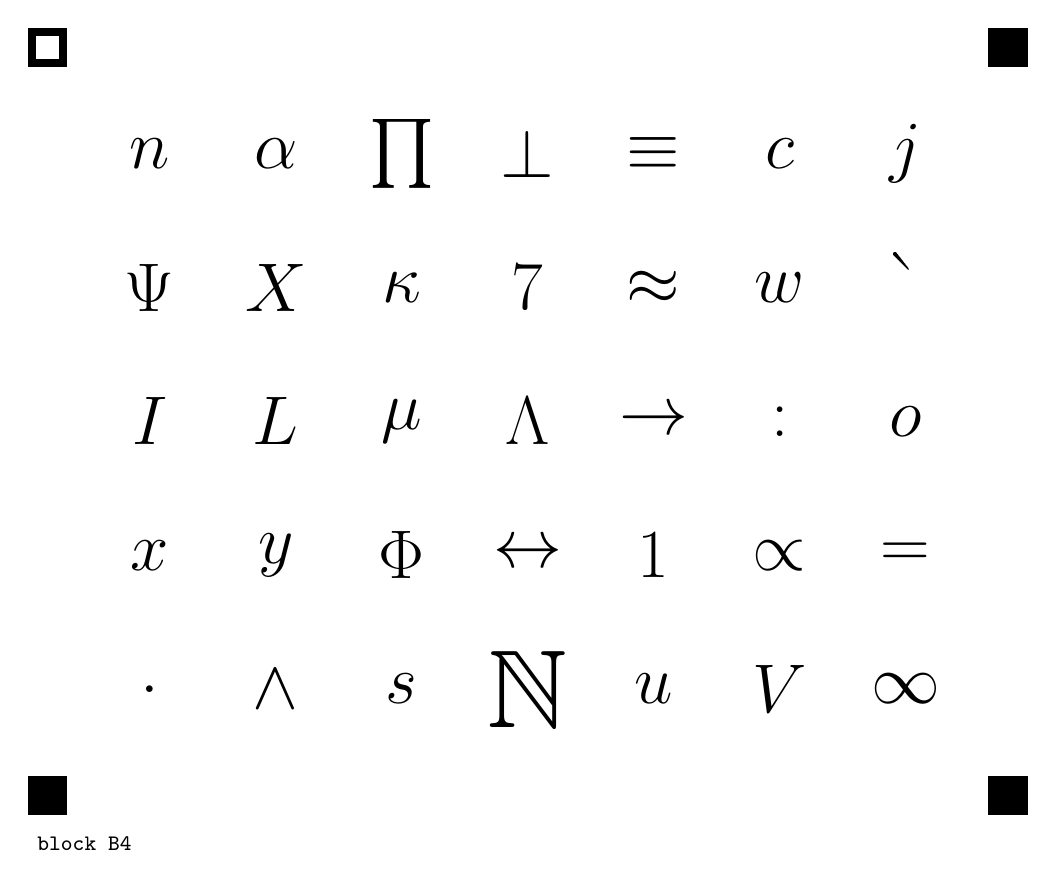
\begin{tikzpicture}[x=1cm,y=-1cm]
\draw[line width=1mm] (-0.700,-0.700) rectangle (-0.300,-0.300);
\fill (11.450,-0.750) rectangle ++(0.500,0.500);
\fill (11.450,8.750) rectangle ++(0.500,0.500);
\fill (-0.750,8.750) rectangle ++(0.500,0.500);
\node[inner sep=0pt] at (0.800,0.850) {\fontsize{40}{48}\selectfont $n$};
\node[inner sep=0pt] at (2.400,0.850) {\fontsize{40}{48}\selectfont $\alpha$};
\node[inner sep=0pt] at (4.000,0.850) {\fontsize{40}{48}\selectfont $\prod$};
\node[inner sep=0pt] at (5.600,0.850) {\fontsize{40}{48}\selectfont $\perp$};
\node[inner sep=0pt] at (7.200,0.850) {\fontsize{40}{48}\selectfont $\equiv$};
\node[inner sep=0pt] at (8.800,0.850) {\fontsize{40}{48}\selectfont $c$};
\node[inner sep=0pt] at (10.400,0.850) {\fontsize{40}{48}\selectfont $j$};
\node[inner sep=0pt] at (0.800,2.550) {\fontsize{40}{48}\selectfont $\Psi$};
\node[inner sep=0pt] at (2.400,2.550) {\fontsize{40}{48}\selectfont $X$};
\node[inner sep=0pt] at (4.000,2.550) {\fontsize{40}{48}\selectfont $\kappa$};
\node[inner sep=0pt] at (5.600,2.550) {\fontsize{40}{48}\selectfont $7$};
\node[inner sep=0pt] at (7.200,2.550) {\fontsize{40}{48}\selectfont $\approx$};
\node[inner sep=0pt] at (8.800,2.550) {\fontsize{40}{48}\selectfont $w$};
\node[inner sep=0pt] at (10.400,2.550) {\fontsize{40}{48}\selectfont $\text{\textasciigrave}$};
\node[inner sep=0pt] at (0.800,4.250) {\fontsize{40}{48}\selectfont $I$};
\node[inner sep=0pt] at (2.400,4.250) {\fontsize{40}{48}\selectfont $L$};
\node[inner sep=0pt] at (4.000,4.250) {\fontsize{40}{48}\selectfont $\mu$};
\node[inner sep=0pt] at (5.600,4.250) {\fontsize{40}{48}\selectfont $\Lambda$};
\node[inner sep=0pt] at (7.200,4.250) {\fontsize{40}{48}\selectfont $\rightarrow$};
\node[inner sep=0pt] at (8.800,4.250) {\fontsize{40}{48}\selectfont $:$};
\node[inner sep=0pt] at (10.400,4.250) {\fontsize{40}{48}\selectfont $o$};
\node[inner sep=0pt] at (0.800,5.950) {\fontsize{40}{48}\selectfont $x$};
\node[inner sep=0pt] at (2.400,5.950) {\fontsize{40}{48}\selectfont $y$};
\node[inner sep=0pt] at (4.000,5.950) {\fontsize{40}{48}\selectfont $\Phi$};
\node[inner sep=0pt] at (5.600,5.950) {\fontsize{40}{48}\selectfont $\leftrightarrow$};
\node[inner sep=0pt] at (7.200,5.950) {\fontsize{40}{48}\selectfont $1$};
\node[inner sep=0pt] at (8.800,5.950) {\fontsize{40}{48}\selectfont $\propto$};
\node[inner sep=0pt] at (10.400,5.950) {\fontsize{40}{48}\selectfont $=$};
\node[inner sep=0pt] at (0.800,7.650) {\fontsize{40}{48}\selectfont $.$};
\node[inner sep=0pt] at (2.400,7.650) {\fontsize{40}{48}\selectfont $\wedge$};
\node[inner sep=0pt] at (4.000,7.650) {\fontsize{40}{48}\selectfont $s$};
\node[inner sep=0pt] at (5.600,7.650) {\fontsize{40}{48}\selectfont $\mathbb{N}$};
\node[inner sep=0pt] at (7.200,7.650) {\fontsize{40}{48}\selectfont $u$};
\node[inner sep=0pt] at (8.800,7.650) {\fontsize{40}{48}\selectfont $V$};
\node[inner sep=0pt] at (10.400,7.650) {\fontsize{40}{48}\selectfont $\infty$};
\node[anchor=north west,font=\footnotesize\ttfamily] at (-0.750,9.400) {block B4};
\end{tikzpicture}\end{center}\vspace{0.2cm}
\newpage
{\small Camera-to-LaTeX data sheet. Print at 100\,\%. Photograph each block 3 times with all four corner squares in view; the hollow square goes top left.}\par\vspace{0.3cm}
\begin{center}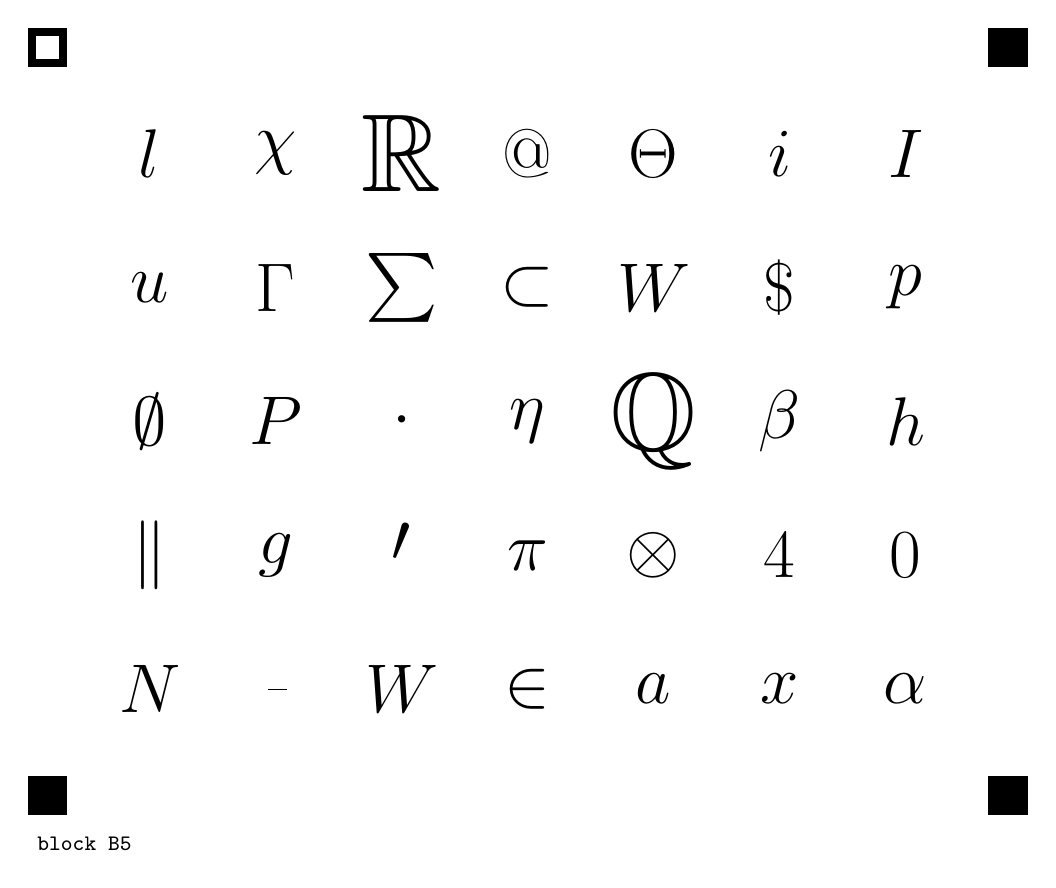
\begin{tikzpicture}[x=1cm,y=-1cm]
\draw[line width=1mm] (-0.700,-0.700) rectangle (-0.300,-0.300);
\fill (11.450,-0.750) rectangle ++(0.500,0.500);
\fill (11.450,8.750) rectangle ++(0.500,0.500);
\fill (-0.750,8.750) rectangle ++(0.500,0.500);
\node[inner sep=0pt] at (0.800,0.850) {\fontsize{40}{48}\selectfont $l$};
\node[inner sep=0pt] at (2.400,0.850) {\fontsize{40}{48}\selectfont $\chi$};
\node[inner sep=0pt] at (4.000,0.850) {\fontsize{40}{48}\selectfont $\mathbb{R}$};
\node[inner sep=0pt] at (5.600,0.850) {\fontsize{40}{48}\selectfont $@$};
\node[inner sep=0pt] at (7.200,0.850) {\fontsize{40}{48}\selectfont $\Theta$};
\node[inner sep=0pt] at (8.800,0.850) {\fontsize{40}{48}\selectfont $i$};
\node[inner sep=0pt] at (10.400,0.850) {\fontsize{40}{48}\selectfont $I$};
\node[inner sep=0pt] at (0.800,2.550) {\fontsize{40}{48}\selectfont $u$};
\node[inner sep=0pt] at (2.400,2.550) {\fontsize{40}{48}\selectfont $\Gamma$};
\node[inner sep=0pt] at (4.000,2.550) {\fontsize{40}{48}\selectfont $\sum$};
\node[inner sep=0pt] at (5.600,2.550) {\fontsize{40}{48}\selectfont $\subset$};
\node[inner sep=0pt] at (7.200,2.550) {\fontsize{40}{48}\selectfont $W$};
\node[inner sep=0pt] at (8.800,2.550) {\fontsize{40}{48}\selectfont $\$$};
\node[inner sep=0pt] at (10.400,2.550) {\fontsize{40}{48}\selectfont $p$};
\node[inner sep=0pt] at (0.800,4.250) {\fontsize{40}{48}\selectfont $\emptyset$};
\node[inner sep=0pt] at (2.400,4.250) {\fontsize{40}{48}\selectfont $P$};
\node[inner sep=0pt] at (4.000,4.250) {\fontsize{40}{48}\selectfont $\cdot$};
\node[inner sep=0pt] at (5.600,4.250) {\fontsize{40}{48}\selectfont $\eta$};
\node[inner sep=0pt] at (7.200,4.250) {\fontsize{40}{48}\selectfont $\mathbb{Q}$};
\node[inner sep=0pt] at (8.800,4.250) {\fontsize{40}{48}\selectfont $\beta$};
\node[inner sep=0pt] at (10.400,4.250) {\fontsize{40}{48}\selectfont $h$};
\node[inner sep=0pt] at (0.800,5.950) {\fontsize{40}{48}\selectfont $\parallel$};
\node[inner sep=0pt] at (2.400,5.950) {\fontsize{40}{48}\selectfont $g$};
\node[inner sep=0pt] at (4.000,5.950) {\fontsize{40}{48}\selectfont $'$};
\node[inner sep=0pt] at (5.600,5.950) {\fontsize{40}{48}\selectfont $\pi$};
\node[inner sep=0pt] at (7.200,5.950) {\fontsize{40}{48}\selectfont $\otimes$};
\node[inner sep=0pt] at (8.800,5.950) {\fontsize{40}{48}\selectfont $4$};
\node[inner sep=0pt] at (10.400,5.950) {\fontsize{40}{48}\selectfont $0$};
\node[inner sep=0pt] at (0.800,7.650) {\fontsize{40}{48}\selectfont $N$};
\node[inner sep=0pt] at (2.400,7.650) {\fontsize{40}{48}\selectfont $\_$};
\node[inner sep=0pt] at (4.000,7.650) {\fontsize{40}{48}\selectfont $W$};
\node[inner sep=0pt] at (5.600,7.650) {\fontsize{40}{48}\selectfont $\in$};
\node[inner sep=0pt] at (7.200,7.650) {\fontsize{40}{48}\selectfont $a$};
\node[inner sep=0pt] at (8.800,7.650) {\fontsize{40}{48}\selectfont $x$};
\node[inner sep=0pt] at (10.400,7.650) {\fontsize{40}{48}\selectfont $\alpha$};
\node[anchor=north west,font=\footnotesize\ttfamily] at (-0.750,9.400) {block B5};
\end{tikzpicture}\end{center}\vspace{0.2cm}
\begin{center}\begin{tikzpicture}[x=1cm,y=-1cm]
\draw[line width=1mm] (-0.700,-0.700) rectangle (-0.300,-0.300);
\fill (11.450,-0.750) rectangle ++(0.500,0.500);
\fill (11.450,8.750) rectangle ++(0.500,0.500);
\fill (-0.750,8.750) rectangle ++(0.500,0.500);
\node[inner sep=0pt] at (0.800,0.850) {\fontsize{40}{48}\selectfont $\zeta$};
\node[inner sep=0pt] at (2.400,0.850) {\fontsize{40}{48}\selectfont $w$};
\node[inner sep=0pt] at (4.000,0.850) {\fontsize{40}{48}\selectfont $a$};
\node[inner sep=0pt] at (5.600,0.850) {\fontsize{40}{48}\selectfont $G$};
\node[inner sep=0pt] at (7.200,0.850) {\fontsize{40}{48}\selectfont $\neg$};
\node[inner sep=0pt] at (8.800,0.850) {\fontsize{40}{48}\selectfont $\oplus$};
\node[inner sep=0pt] at (10.400,0.850) {\fontsize{40}{48}\selectfont $\Leftrightarrow$};
\node[inner sep=0pt] at (0.800,2.550) {\fontsize{40}{48}\selectfont $m$};
\node[inner sep=0pt] at (2.400,2.550) {\fontsize{40}{48}\selectfont $\hbar$};
\node[inner sep=0pt] at (4.000,2.550) {\fontsize{40}{48}\selectfont $+$};
\node[inner sep=0pt] at (5.600,2.550) {\fontsize{40}{48}\selectfont $\cup$};
\node[inner sep=0pt] at (7.200,2.550) {\fontsize{40}{48}\selectfont $\}$};
\node[inner sep=0pt] at (8.800,2.550) {\fontsize{40}{48}\selectfont $\phi$};
\node[inner sep=0pt] at (10.400,2.550) {\fontsize{40}{48}\selectfont $8$};
\node[inner sep=0pt] at (0.800,4.250) {\fontsize{40}{48}\selectfont $H$};
\node[inner sep=0pt] at (2.400,4.250) {\fontsize{40}{48}\selectfont $*$};
\node[inner sep=0pt] at (4.000,4.250) {\fontsize{40}{48}\selectfont $\neq$};
\node[inner sep=0pt] at (5.600,4.250) {\fontsize{40}{48}\selectfont $k$};
\node[inner sep=0pt] at (7.200,4.250) {\fontsize{40}{48}\selectfont $\times$};
\node[inner sep=0pt] at (8.800,4.250) {\fontsize{40}{48}\selectfont $\backslash$};
\node[inner sep=0pt] at (10.400,4.250) {\fontsize{40}{48}\selectfont $t$};
\node[inner sep=0pt] at (0.800,5.950) {\fontsize{40}{48}\selectfont $,$};
\node[inner sep=0pt] at (2.400,5.950) {\fontsize{40}{48}\selectfont $\tau$};
\node[inner sep=0pt] at (4.000,5.950) {\fontsize{40}{48}\selectfont $d$};
\node[inner sep=0pt] at (5.600,5.950) {\fontsize{40}{48}\selectfont $\ell$};
\node[inner sep=0pt] at (7.200,5.950) {\fontsize{40}{48}\selectfont $\geq$};
\node[inner sep=0pt] at (8.800,5.950) {\fontsize{40}{48}\selectfont $M$};
\node[inner sep=0pt] at (10.400,5.950) {\fontsize{40}{48}\selectfont $\text{\textquotedbl}$};
\node[inner sep=0pt] at (0.800,7.650) {\fontsize{40}{48}\selectfont $\nabla$};
\node[inner sep=0pt] at (2.400,7.650) {\fontsize{40}{48}\selectfont $^{\circ}$};
\node[inner sep=0pt] at (4.000,7.650) {\fontsize{40}{48}\selectfont $\sim$};
\node[inner sep=0pt] at (5.600,7.650) {\fontsize{40}{48}\selectfont $\exists$};
\node[inner sep=0pt] at (7.200,7.650) {\fontsize{40}{48}\selectfont $<$};
\node[inner sep=0pt] at (8.800,7.650) {\fontsize{40}{48}\selectfont $\Sigma$};
\node[inner sep=0pt] at (10.400,7.650) {\fontsize{40}{48}\selectfont $\gg$};
\node[anchor=north west,font=\footnotesize\ttfamily] at (-0.750,9.400) {block B6};
\end{tikzpicture}\end{center}\vspace{0.2cm}
\newpage
{\small Camera-to-LaTeX data sheet. Print at 100\,\%. Photograph each block 3 times with all four corner squares in view; the hollow square goes top left.}\par\vspace{0.3cm}
\begin{center}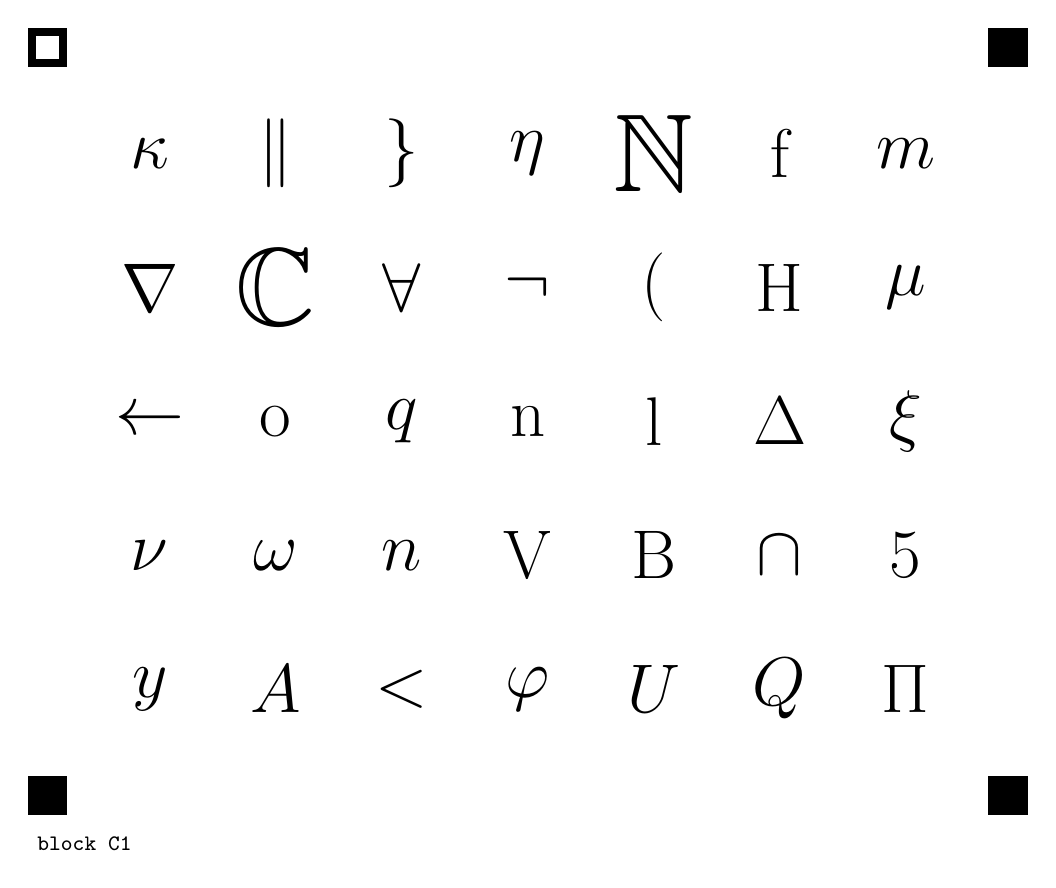
\begin{tikzpicture}[x=1cm,y=-1cm]
\draw[line width=1mm] (-0.700,-0.700) rectangle (-0.300,-0.300);
\fill (11.450,-0.750) rectangle ++(0.500,0.500);
\fill (11.450,8.750) rectangle ++(0.500,0.500);
\fill (-0.750,8.750) rectangle ++(0.500,0.500);
\node[inner sep=0pt] at (0.800,0.850) {\fontsize{40}{48}\selectfont $\kappa$};
\node[inner sep=0pt] at (2.400,0.850) {\fontsize{40}{48}\selectfont $\parallel$};
\node[inner sep=0pt] at (4.000,0.850) {\fontsize{40}{48}\selectfont \}};
\node[inner sep=0pt] at (5.600,0.850) {\fontsize{40}{48}\selectfont $\eta$};
\node[inner sep=0pt] at (7.200,0.850) {\fontsize{40}{48}\selectfont $\mathbb{N}$};
\node[inner sep=0pt] at (8.800,0.850) {\fontsize{40}{48}\selectfont f};
\node[inner sep=0pt] at (10.400,0.850) {\fontsize{40}{48}\selectfont $m$};
\node[inner sep=0pt] at (0.800,2.550) {\fontsize{40}{48}\selectfont $\nabla$};
\node[inner sep=0pt] at (2.400,2.550) {\fontsize{40}{48}\selectfont $\mathbb{C}$};
\node[inner sep=0pt] at (4.000,2.550) {\fontsize{40}{48}\selectfont $\forall$};
\node[inner sep=0pt] at (5.600,2.550) {\fontsize{40}{48}\selectfont $\neg$};
\node[inner sep=0pt] at (7.200,2.550) {\fontsize{40}{48}\selectfont $($};
\node[inner sep=0pt] at (8.800,2.550) {\fontsize{40}{48}\selectfont H};
\node[inner sep=0pt] at (10.400,2.550) {\fontsize{40}{48}\selectfont $\mu$};
\node[inner sep=0pt] at (0.800,4.250) {\fontsize{40}{48}\selectfont $\leftarrow$};
\node[inner sep=0pt] at (2.400,4.250) {\fontsize{40}{48}\selectfont o};
\node[inner sep=0pt] at (4.000,4.250) {\fontsize{40}{48}\selectfont $q$};
\node[inner sep=0pt] at (5.600,4.250) {\fontsize{40}{48}\selectfont n};
\node[inner sep=0pt] at (7.200,4.250) {\fontsize{40}{48}\selectfont l};
\node[inner sep=0pt] at (8.800,4.250) {\fontsize{40}{48}\selectfont $\Delta$};
\node[inner sep=0pt] at (10.400,4.250) {\fontsize{40}{48}\selectfont $\xi$};
\node[inner sep=0pt] at (0.800,5.950) {\fontsize{40}{48}\selectfont $\nu$};
\node[inner sep=0pt] at (2.400,5.950) {\fontsize{40}{48}\selectfont $\omega$};
\node[inner sep=0pt] at (4.000,5.950) {\fontsize{40}{48}\selectfont $n$};
\node[inner sep=0pt] at (5.600,5.950) {\fontsize{40}{48}\selectfont V};
\node[inner sep=0pt] at (7.200,5.950) {\fontsize{40}{48}\selectfont B};
\node[inner sep=0pt] at (8.800,5.950) {\fontsize{40}{48}\selectfont $\cap$};
\node[inner sep=0pt] at (10.400,5.950) {\fontsize{40}{48}\selectfont $5$};
\node[inner sep=0pt] at (0.800,7.650) {\fontsize{40}{48}\selectfont $y$};
\node[inner sep=0pt] at (2.400,7.650) {\fontsize{40}{48}\selectfont $A$};
\node[inner sep=0pt] at (4.000,7.650) {\fontsize{40}{48}\selectfont \textless{}};
\node[inner sep=0pt] at (5.600,7.650) {\fontsize{40}{48}\selectfont $\varphi$};
\node[inner sep=0pt] at (7.200,7.650) {\fontsize{40}{48}\selectfont $U$};
\node[inner sep=0pt] at (8.800,7.650) {\fontsize{40}{48}\selectfont $Q$};
\node[inner sep=0pt] at (10.400,7.650) {\fontsize{40}{48}\selectfont $\Pi$};
\node[anchor=north west,font=\footnotesize\ttfamily] at (-0.750,9.400) {block C1};
\end{tikzpicture}\end{center}\vspace{0.2cm}
\begin{center}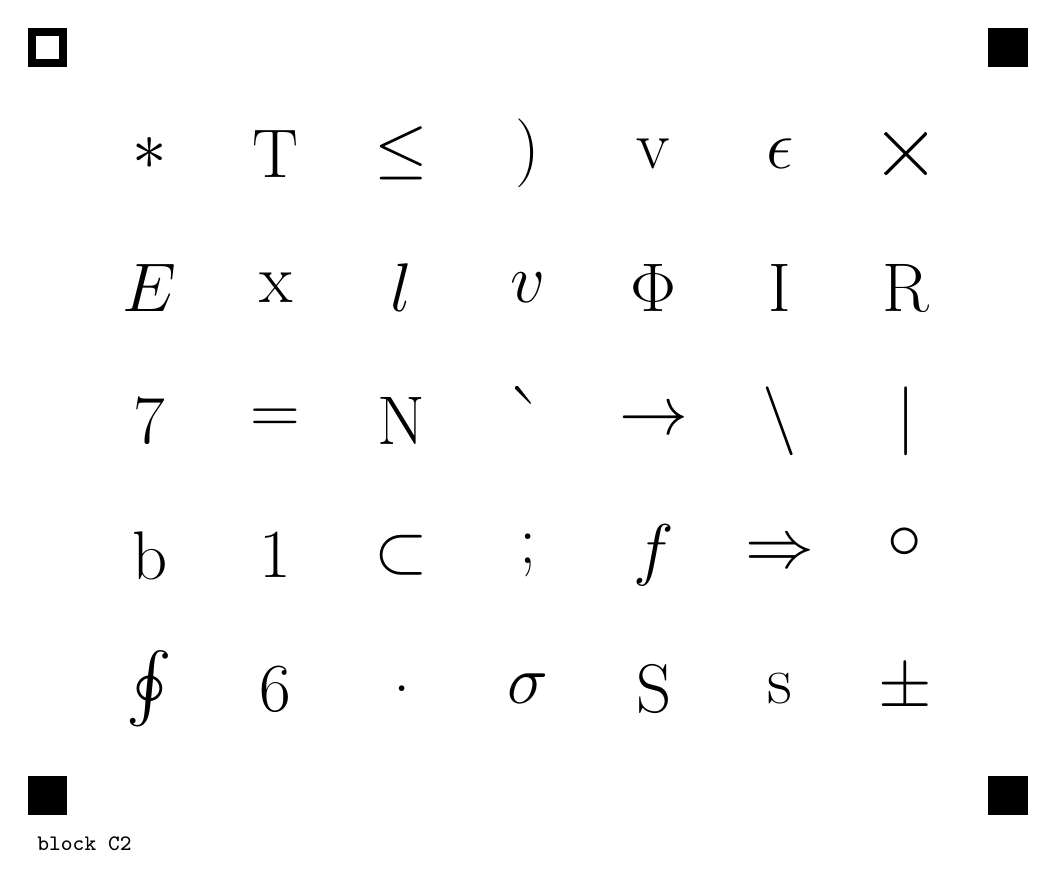
\begin{tikzpicture}[x=1cm,y=-1cm]
\draw[line width=1mm] (-0.700,-0.700) rectangle (-0.300,-0.300);
\fill (11.450,-0.750) rectangle ++(0.500,0.500);
\fill (11.450,8.750) rectangle ++(0.500,0.500);
\fill (-0.750,8.750) rectangle ++(0.500,0.500);
\node[inner sep=0pt] at (0.800,0.850) {\fontsize{40}{48}\selectfont $*$};
\node[inner sep=0pt] at (2.400,0.850) {\fontsize{40}{48}\selectfont T};
\node[inner sep=0pt] at (4.000,0.850) {\fontsize{40}{48}\selectfont $\leq$};
\node[inner sep=0pt] at (5.600,0.850) {\fontsize{40}{48}\selectfont $)$};
\node[inner sep=0pt] at (7.200,0.850) {\fontsize{40}{48}\selectfont v};
\node[inner sep=0pt] at (8.800,0.850) {\fontsize{40}{48}\selectfont $\epsilon$};
\node[inner sep=0pt] at (10.400,0.850) {\fontsize{40}{48}\selectfont \texttimes{}};
\node[inner sep=0pt] at (0.800,2.550) {\fontsize{40}{48}\selectfont $E$};
\node[inner sep=0pt] at (2.400,2.550) {\fontsize{40}{48}\selectfont x};
\node[inner sep=0pt] at (4.000,2.550) {\fontsize{40}{48}\selectfont $l$};
\node[inner sep=0pt] at (5.600,2.550) {\fontsize{40}{48}\selectfont $v$};
\node[inner sep=0pt] at (7.200,2.550) {\fontsize{40}{48}\selectfont $\Phi$};
\node[inner sep=0pt] at (8.800,2.550) {\fontsize{40}{48}\selectfont I};
\node[inner sep=0pt] at (10.400,2.550) {\fontsize{40}{48}\selectfont R};
\node[inner sep=0pt] at (0.800,4.250) {\fontsize{40}{48}\selectfont 7};
\node[inner sep=0pt] at (2.400,4.250) {\fontsize{40}{48}\selectfont $=$};
\node[inner sep=0pt] at (4.000,4.250) {\fontsize{40}{48}\selectfont N};
\node[inner sep=0pt] at (5.600,4.250) {\fontsize{40}{48}\selectfont \textasciigrave{}};
\node[inner sep=0pt] at (7.200,4.250) {\fontsize{40}{48}\selectfont $\rightarrow$};
\node[inner sep=0pt] at (8.800,4.250) {\fontsize{40}{48}\selectfont \textbackslash{}};
\node[inner sep=0pt] at (10.400,4.250) {\fontsize{40}{48}\selectfont \textbar{}};
\node[inner sep=0pt] at (0.800,5.950) {\fontsize{40}{48}\selectfont b};
\node[inner sep=0pt] at (2.400,5.950) {\fontsize{40}{48}\selectfont 1};
\node[inner sep=0pt] at (4.000,5.950) {\fontsize{40}{48}\selectfont $\subset$};
\node[inner sep=0pt] at (5.600,5.950) {\fontsize{40}{48}\selectfont ;};
\node[inner sep=0pt] at (7.200,5.950) {\fontsize{40}{48}\selectfont $f$};
\node[inner sep=0pt] at (8.800,5.950) {\fontsize{40}{48}\selectfont $\Rightarrow$};
\node[inner sep=0pt] at (10.400,5.950) {\fontsize{40}{48}\selectfont $^{\circ}$};
\node[inner sep=0pt] at (0.800,7.650) {\fontsize{40}{48}\selectfont $\oint$};
\node[inner sep=0pt] at (2.400,7.650) {\fontsize{40}{48}\selectfont $6$};
\node[inner sep=0pt] at (4.000,7.650) {\fontsize{40}{48}\selectfont .};
\node[inner sep=0pt] at (5.600,7.650) {\fontsize{40}{48}\selectfont $\sigma$};
\node[inner sep=0pt] at (7.200,7.650) {\fontsize{40}{48}\selectfont S};
\node[inner sep=0pt] at (8.800,7.650) {\fontsize{40}{48}\selectfont s};
\node[inner sep=0pt] at (10.400,7.650) {\fontsize{40}{48}\selectfont $\pm$};
\node[anchor=north west,font=\footnotesize\ttfamily] at (-0.750,9.400) {block C2};
\end{tikzpicture}\end{center}\vspace{0.2cm}
\newpage
{\small Camera-to-LaTeX data sheet. Print at 100\,\%. Photograph each block 3 times with all four corner squares in view; the hollow square goes top left.}\par\vspace{0.3cm}
\begin{center}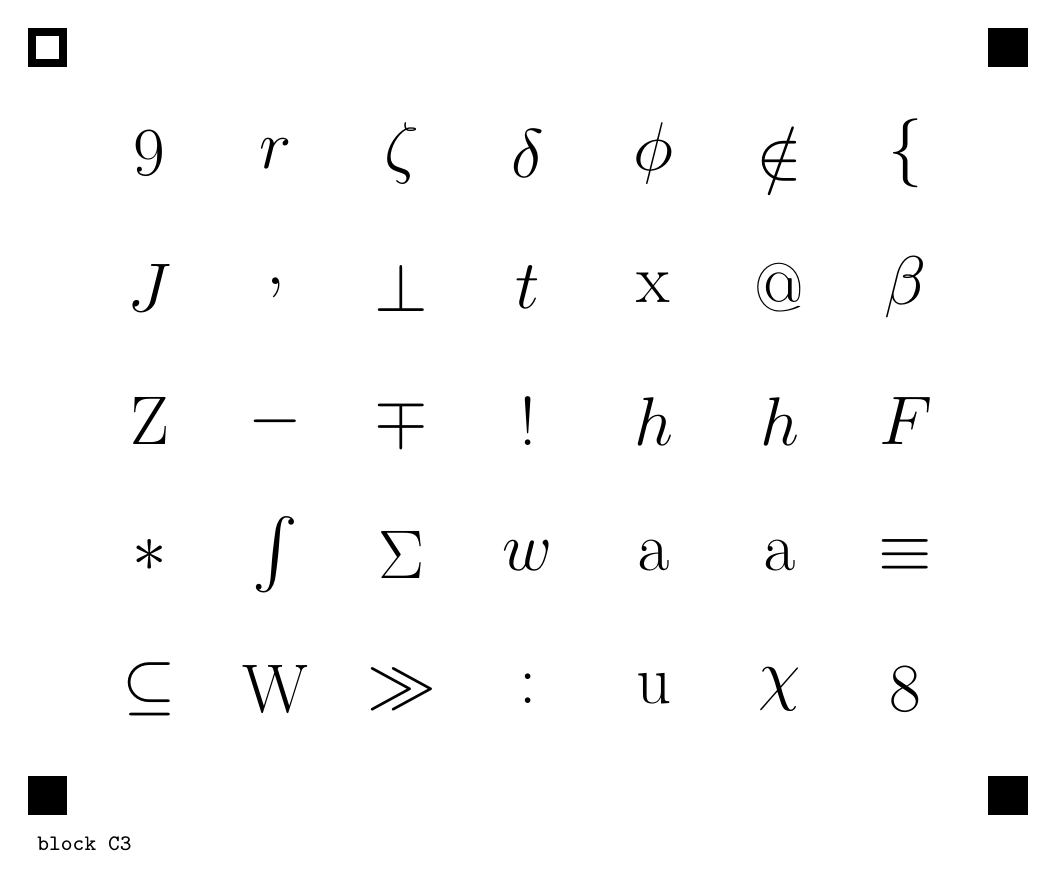
\begin{tikzpicture}[x=1cm,y=-1cm]
\draw[line width=1mm] (-0.700,-0.700) rectangle (-0.300,-0.300);
\fill (11.450,-0.750) rectangle ++(0.500,0.500);
\fill (11.450,8.750) rectangle ++(0.500,0.500);
\fill (-0.750,8.750) rectangle ++(0.500,0.500);
\node[inner sep=0pt] at (0.800,0.850) {\fontsize{40}{48}\selectfont 9};
\node[inner sep=0pt] at (2.400,0.850) {\fontsize{40}{48}\selectfont $r$};
\node[inner sep=0pt] at (4.000,0.850) {\fontsize{40}{48}\selectfont $\zeta$};
\node[inner sep=0pt] at (5.600,0.850) {\fontsize{40}{48}\selectfont $\delta$};
\node[inner sep=0pt] at (7.200,0.850) {\fontsize{40}{48}\selectfont $\phi$};
\node[inner sep=0pt] at (8.800,0.850) {\fontsize{40}{48}\selectfont $\notin$};
\node[inner sep=0pt] at (10.400,0.850) {\fontsize{40}{48}\selectfont \{};
\node[inner sep=0pt] at (0.800,2.550) {\fontsize{40}{48}\selectfont $J$};
\node[inner sep=0pt] at (2.400,2.550) {\fontsize{40}{48}\selectfont $,$};
\node[inner sep=0pt] at (4.000,2.550) {\fontsize{40}{48}\selectfont $\perp$};
\node[inner sep=0pt] at (5.600,2.550) {\fontsize{40}{48}\selectfont $t$};
\node[inner sep=0pt] at (7.200,2.550) {\fontsize{40}{48}\selectfont x};
\node[inner sep=0pt] at (8.800,2.550) {\fontsize{40}{48}\selectfont @};
\node[inner sep=0pt] at (10.400,2.550) {\fontsize{40}{48}\selectfont $\beta$};
\node[inner sep=0pt] at (0.800,4.250) {\fontsize{40}{48}\selectfont Z};
\node[inner sep=0pt] at (2.400,4.250) {\fontsize{40}{48}\selectfont $-$};
\node[inner sep=0pt] at (4.000,4.250) {\fontsize{40}{48}\selectfont $\mp$};
\node[inner sep=0pt] at (5.600,4.250) {\fontsize{40}{48}\selectfont $!$};
\node[inner sep=0pt] at (7.200,4.250) {\fontsize{40}{48}\selectfont $h$};
\node[inner sep=0pt] at (8.800,4.250) {\fontsize{40}{48}\selectfont $h$};
\node[inner sep=0pt] at (10.400,4.250) {\fontsize{40}{48}\selectfont $F$};
\node[inner sep=0pt] at (0.800,5.950) {\fontsize{40}{48}\selectfont $\ast$};
\node[inner sep=0pt] at (2.400,5.950) {\fontsize{40}{48}\selectfont $\int$};
\node[inner sep=0pt] at (4.000,5.950) {\fontsize{40}{48}\selectfont $\Sigma$};
\node[inner sep=0pt] at (5.600,5.950) {\fontsize{40}{48}\selectfont $w$};
\node[inner sep=0pt] at (7.200,5.950) {\fontsize{40}{48}\selectfont a};
\node[inner sep=0pt] at (8.800,5.950) {\fontsize{40}{48}\selectfont a};
\node[inner sep=0pt] at (10.400,5.950) {\fontsize{40}{48}\selectfont $\equiv$};
\node[inner sep=0pt] at (0.800,7.650) {\fontsize{40}{48}\selectfont $\subseteq$};
\node[inner sep=0pt] at (2.400,7.650) {\fontsize{40}{48}\selectfont W};
\node[inner sep=0pt] at (4.000,7.650) {\fontsize{40}{48}\selectfont $\gg$};
\node[inner sep=0pt] at (5.600,7.650) {\fontsize{40}{48}\selectfont $:$};
\node[inner sep=0pt] at (7.200,7.650) {\fontsize{40}{48}\selectfont u};
\node[inner sep=0pt] at (8.800,7.650) {\fontsize{40}{48}\selectfont $\chi$};
\node[inner sep=0pt] at (10.400,7.650) {\fontsize{40}{48}\selectfont $8$};
\node[anchor=north west,font=\footnotesize\ttfamily] at (-0.750,9.400) {block C3};
\end{tikzpicture}\end{center}\vspace{0.2cm}
\begin{center}\begin{tikzpicture}[x=1cm,y=-1cm]
\draw[line width=1mm] (-0.700,-0.700) rectangle (-0.300,-0.300);
\fill (11.450,-0.750) rectangle ++(0.500,0.500);
\fill (11.450,8.750) rectangle ++(0.500,0.500);
\fill (-0.750,8.750) rectangle ++(0.500,0.500);
\node[inner sep=0pt] at (0.800,0.850) {\fontsize{40}{48}\selectfont $\varepsilon$};
\node[inner sep=0pt] at (2.400,0.850) {\fontsize{40}{48}\selectfont \textbar{}};
\node[inner sep=0pt] at (4.000,0.850) {\fontsize{40}{48}\selectfont $\exists$};
\node[inner sep=0pt] at (5.600,0.850) {\fontsize{40}{48}\selectfont \&};
\node[inner sep=0pt] at (7.200,0.850) {\fontsize{40}{48}\selectfont w};
\node[inner sep=0pt] at (8.800,0.850) {\fontsize{40}{48}\selectfont $\hbar$};
\node[inner sep=0pt] at (10.400,0.850) {\fontsize{40}{48}\selectfont $\ell$};
\node[inner sep=0pt] at (0.800,2.550) {\fontsize{40}{48}\selectfont $1$};
\node[inner sep=0pt] at (2.400,2.550) {\fontsize{40}{48}\selectfont $\Xi$};
\node[inner sep=0pt] at (4.000,2.550) {\fontsize{40}{48}\selectfont $\Leftrightarrow$};
\node[inner sep=0pt] at (5.600,2.550) {\fontsize{40}{48}\selectfont $\sum$};
\node[inner sep=0pt] at (7.200,2.550) {\fontsize{40}{48}\selectfont $\vee$};
\node[inner sep=0pt] at (8.800,2.550) {\fontsize{40}{48}\selectfont m};
\node[inner sep=0pt] at (10.400,2.550) {\fontsize{40}{48}\selectfont $\partial$};
\node[inner sep=0pt] at (0.800,4.250) {\fontsize{40}{48}\selectfont O};
\node[inner sep=0pt] at (2.400,4.250) {\fontsize{40}{48}\selectfont ]};
\node[inner sep=0pt] at (4.000,4.250) {\fontsize{40}{48}\selectfont $k$};
\node[inner sep=0pt] at (5.600,4.250) {\fontsize{40}{48}\selectfont $+$};
\node[inner sep=0pt] at (7.200,4.250) {\fontsize{40}{48}\selectfont $e$};
\node[inner sep=0pt] at (8.800,4.250) {\fontsize{40}{48}\selectfont \textquotedbl{}};
\node[inner sep=0pt] at (10.400,4.250) {\fontsize{40}{48}\selectfont \%};
\node[inner sep=0pt] at (0.800,5.950) {\fontsize{40}{48}\selectfont -};
\node[inner sep=0pt] at (2.400,5.950) {\fontsize{40}{48}\selectfont $\propto$};
\node[inner sep=0pt] at (4.000,5.950) {\fontsize{40}{48}\selectfont $,$};
\node[inner sep=0pt] at (5.600,5.950) {\fontsize{40}{48}\selectfont $\mathbb{R}$};
\node[inner sep=0pt] at (7.200,5.950) {\fontsize{40}{48}\selectfont .};
\node[inner sep=0pt] at (8.800,5.950) {\fontsize{40}{48}\selectfont O};
\node[inner sep=0pt] at (10.400,5.950) {\fontsize{40}{48}\selectfont [};
\node[inner sep=0pt] at (0.800,7.650) {\fontsize{40}{48}\selectfont $\pi$};
\node[inner sep=0pt] at (2.400,7.650) {\fontsize{40}{48}\selectfont $d$};
\node[inner sep=0pt] at (4.000,7.650) {\fontsize{40}{48}\selectfont $/$};
\node[inner sep=0pt] at (5.600,7.650) {\fontsize{40}{48}\selectfont $\approx$};
\node[inner sep=0pt] at (7.200,7.650) {\fontsize{40}{48}\selectfont $G$};
\node[inner sep=0pt] at (8.800,7.650) {\fontsize{40}{48}\selectfont 4};
\node[inner sep=0pt] at (10.400,7.650) {\fontsize{40}{48}\selectfont $\geq$};
\node[anchor=north west,font=\footnotesize\ttfamily] at (-0.750,9.400) {block C4};
\end{tikzpicture}\end{center}\vspace{0.2cm}
\newpage
{\small Camera-to-LaTeX data sheet. Print at 100\,\%. Photograph each block 3 times with all four corner squares in view; the hollow square goes top left.}\par\vspace{0.3cm}
\begin{center}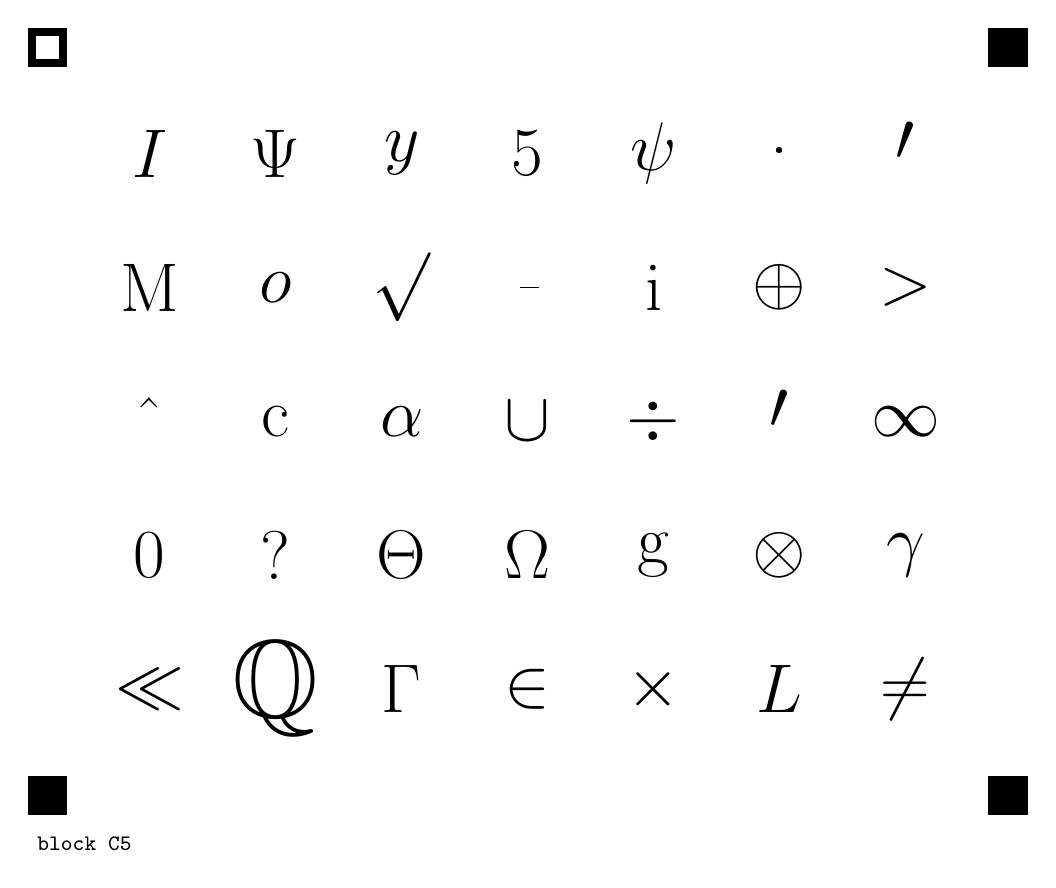
\begin{tikzpicture}[x=1cm,y=-1cm]
\draw[line width=1mm] (-0.700,-0.700) rectangle (-0.300,-0.300);
\fill (11.450,-0.750) rectangle ++(0.500,0.500);
\fill (11.450,8.750) rectangle ++(0.500,0.500);
\fill (-0.750,8.750) rectangle ++(0.500,0.500);
\node[inner sep=0pt] at (0.800,0.850) {\fontsize{40}{48}\selectfont $I$};
\node[inner sep=0pt] at (2.400,0.850) {\fontsize{40}{48}\selectfont $\Psi$};
\node[inner sep=0pt] at (4.000,0.850) {\fontsize{40}{48}\selectfont $y$};
\node[inner sep=0pt] at (5.600,0.850) {\fontsize{40}{48}\selectfont $5$};
\node[inner sep=0pt] at (7.200,0.850) {\fontsize{40}{48}\selectfont $\psi$};
\node[inner sep=0pt] at (8.800,0.850) {\fontsize{40}{48}\selectfont \textperiodcentered{}};
\node[inner sep=0pt] at (10.400,0.850) {\fontsize{40}{48}\selectfont $'$};
\node[inner sep=0pt] at (0.800,2.550) {\fontsize{40}{48}\selectfont M};
\node[inner sep=0pt] at (2.400,2.550) {\fontsize{40}{48}\selectfont $o$};
\node[inner sep=0pt] at (4.000,2.550) {\fontsize{40}{48}\selectfont $\surd$};
\node[inner sep=0pt] at (5.600,2.550) {\fontsize{40}{48}\selectfont $\_$};
\node[inner sep=0pt] at (7.200,2.550) {\fontsize{40}{48}\selectfont i};
\node[inner sep=0pt] at (8.800,2.550) {\fontsize{40}{48}\selectfont $\oplus$};
\node[inner sep=0pt] at (10.400,2.550) {\fontsize{40}{48}\selectfont $>$};
\node[inner sep=0pt] at (0.800,4.250) {\fontsize{40}{48}\selectfont $\text{\textasciicircum}$};
\node[inner sep=0pt] at (2.400,4.250) {\fontsize{40}{48}\selectfont c};
\node[inner sep=0pt] at (4.000,4.250) {\fontsize{40}{48}\selectfont $\alpha$};
\node[inner sep=0pt] at (5.600,4.250) {\fontsize{40}{48}\selectfont $\cup$};
\node[inner sep=0pt] at (7.200,4.250) {\fontsize{40}{48}\selectfont $\div$};
\node[inner sep=0pt] at (8.800,4.250) {\fontsize{40}{48}\selectfont $'$};
\node[inner sep=0pt] at (10.400,4.250) {\fontsize{40}{48}\selectfont $\infty$};
\node[inner sep=0pt] at (0.800,5.950) {\fontsize{40}{48}\selectfont $0$};
\node[inner sep=0pt] at (2.400,5.950) {\fontsize{40}{48}\selectfont $?$};
\node[inner sep=0pt] at (4.000,5.950) {\fontsize{40}{48}\selectfont $\Theta$};
\node[inner sep=0pt] at (5.600,5.950) {\fontsize{40}{48}\selectfont $\Omega$};
\node[inner sep=0pt] at (7.200,5.950) {\fontsize{40}{48}\selectfont g};
\node[inner sep=0pt] at (8.800,5.950) {\fontsize{40}{48}\selectfont $\otimes$};
\node[inner sep=0pt] at (10.400,5.950) {\fontsize{40}{48}\selectfont $\gamma$};
\node[inner sep=0pt] at (0.800,7.650) {\fontsize{40}{48}\selectfont $\ll$};
\node[inner sep=0pt] at (2.400,7.650) {\fontsize{40}{48}\selectfont $\mathbb{Q}$};
\node[inner sep=0pt] at (4.000,7.650) {\fontsize{40}{48}\selectfont $\Gamma$};
\node[inner sep=0pt] at (5.600,7.650) {\fontsize{40}{48}\selectfont $\in$};
\node[inner sep=0pt] at (7.200,7.650) {\fontsize{40}{48}\selectfont $\times$};
\node[inner sep=0pt] at (8.800,7.650) {\fontsize{40}{48}\selectfont $L$};
\node[inner sep=0pt] at (10.400,7.650) {\fontsize{40}{48}\selectfont $\neq$};
\node[anchor=north west,font=\footnotesize\ttfamily] at (-0.750,9.400) {block C5};
\end{tikzpicture}\end{center}\vspace{0.2cm}
\begin{center}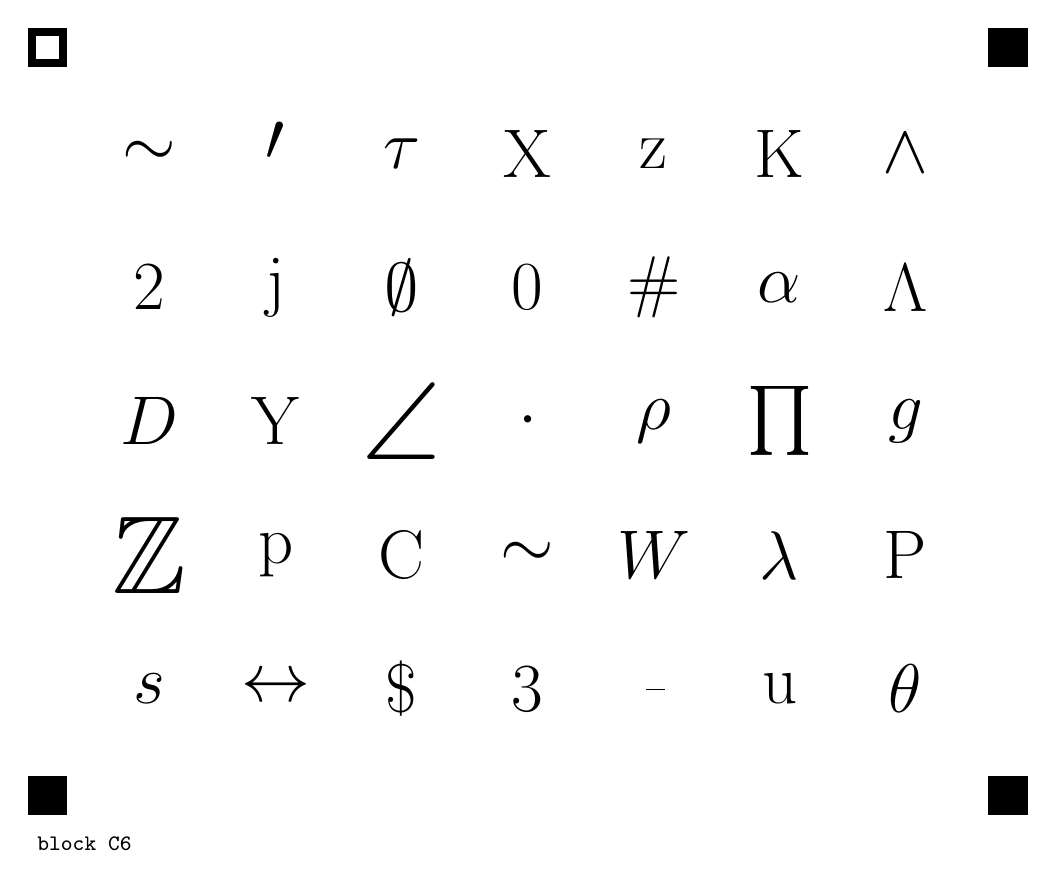
\begin{tikzpicture}[x=1cm,y=-1cm]
\draw[line width=1mm] (-0.700,-0.700) rectangle (-0.300,-0.300);
\fill (11.450,-0.750) rectangle ++(0.500,0.500);
\fill (11.450,8.750) rectangle ++(0.500,0.500);
\fill (-0.750,8.750) rectangle ++(0.500,0.500);
\node[inner sep=0pt] at (0.800,0.850) {\fontsize{40}{48}\selectfont $\sim$};
\node[inner sep=0pt] at (2.400,0.850) {\fontsize{40}{48}\selectfont $'$};
\node[inner sep=0pt] at (4.000,0.850) {\fontsize{40}{48}\selectfont $\tau$};
\node[inner sep=0pt] at (5.600,0.850) {\fontsize{40}{48}\selectfont X};
\node[inner sep=0pt] at (7.200,0.850) {\fontsize{40}{48}\selectfont z};
\node[inner sep=0pt] at (8.800,0.850) {\fontsize{40}{48}\selectfont K};
\node[inner sep=0pt] at (10.400,0.850) {\fontsize{40}{48}\selectfont $\wedge$};
\node[inner sep=0pt] at (0.800,2.550) {\fontsize{40}{48}\selectfont $2$};
\node[inner sep=0pt] at (2.400,2.550) {\fontsize{40}{48}\selectfont j};
\node[inner sep=0pt] at (4.000,2.550) {\fontsize{40}{48}\selectfont $\emptyset$};
\node[inner sep=0pt] at (5.600,2.550) {\fontsize{40}{48}\selectfont 0};
\node[inner sep=0pt] at (7.200,2.550) {\fontsize{40}{48}\selectfont $\#$};
\node[inner sep=0pt] at (8.800,2.550) {\fontsize{40}{48}\selectfont $\alpha$};
\node[inner sep=0pt] at (10.400,2.550) {\fontsize{40}{48}\selectfont $\Lambda$};
\node[inner sep=0pt] at (0.800,4.250) {\fontsize{40}{48}\selectfont $D$};
\node[inner sep=0pt] at (2.400,4.250) {\fontsize{40}{48}\selectfont Y};
\node[inner sep=0pt] at (4.000,4.250) {\fontsize{40}{48}\selectfont $\angle$};
\node[inner sep=0pt] at (5.600,4.250) {\fontsize{40}{48}\selectfont $\cdot$};
\node[inner sep=0pt] at (7.200,4.250) {\fontsize{40}{48}\selectfont $\rho$};
\node[inner sep=0pt] at (8.800,4.250) {\fontsize{40}{48}\selectfont $\prod$};
\node[inner sep=0pt] at (10.400,4.250) {\fontsize{40}{48}\selectfont $g$};
\node[inner sep=0pt] at (0.800,5.950) {\fontsize{40}{48}\selectfont $\mathbb{Z}$};
\node[inner sep=0pt] at (2.400,5.950) {\fontsize{40}{48}\selectfont p};
\node[inner sep=0pt] at (4.000,5.950) {\fontsize{40}{48}\selectfont C};
\node[inner sep=0pt] at (5.600,5.950) {\fontsize{40}{48}\selectfont $\sim$};
\node[inner sep=0pt] at (7.200,5.950) {\fontsize{40}{48}\selectfont $W$};
\node[inner sep=0pt] at (8.800,5.950) {\fontsize{40}{48}\selectfont $\lambda$};
\node[inner sep=0pt] at (10.400,5.950) {\fontsize{40}{48}\selectfont P};
\node[inner sep=0pt] at (0.800,7.650) {\fontsize{40}{48}\selectfont $s$};
\node[inner sep=0pt] at (2.400,7.650) {\fontsize{40}{48}\selectfont $\leftrightarrow$};
\node[inner sep=0pt] at (4.000,7.650) {\fontsize{40}{48}\selectfont $\$$};
\node[inner sep=0pt] at (5.600,7.650) {\fontsize{40}{48}\selectfont 3};
\node[inner sep=0pt] at (7.200,7.650) {\fontsize{40}{48}\selectfont $\_$};
\node[inner sep=0pt] at (8.800,7.650) {\fontsize{40}{48}\selectfont u};
\node[inner sep=0pt] at (10.400,7.650) {\fontsize{40}{48}\selectfont $\theta$};
\node[anchor=north west,font=\footnotesize\ttfamily] at (-0.750,9.400) {block C6};
\end{tikzpicture}\end{center}\vspace{0.2cm}
\end{document}